\documentclass[a4paper,11pt]{article}
\usepackage[paper=a4paper, left=1.5cm, right=1.5cm, bottom=1.5cm, top=1.5cm]{geometry}
\usepackage{ucs}
\usepackage[utf8x]{inputenc}
\usepackage{amsmath}
\usepackage{amsfonts}
\usepackage{amssymb}
\usepackage{amsthm}
\usepackage[latin,spanish]{babel}
\usepackage{fontenc}
\usepackage{graphicx}
%\usepackage{epstopdf}
\usepackage{caratula}

% \usepackage{algpseudocode}
% \usepackage{algorithmicx}
% \usepackage{color}
% \usepackage{pdfpages}
% \usepackage{tikz}
%%%%%% Si se usa tikz para dibujar digrafos, cuando pongas flechas, tira un conflicto. Se soluciona con estas dos lineas:
% \usepackage[matrix,arrow]{xy}
% \usetikzlibrary{intersections}

% \usepackage{dsfont}
% \newcommand{\real}{\mathds{R}}
% \newcommand{\nat}{\mathds{N}}
% \newcommand{\complejos}{\mathds{C}}
% \newcommand{\Subesp}{\mathds{S}}

\usepackage{hyperref}
\hypersetup{%
 % Para que el PDF se abra a pagina completa.
  pdfstartview= {FitH \hypercalcbp{\paperheight-\topmargin-1in-\headheight}},
  pdfauthor={Gaston Requeni},
  pdfsubject={Preinforme - Final Orga2},
 %pdfkeywords={keyword1} {key2} {key3},
 colorlinks=true,
  linkcolor=black,
  urlcolor=blue
}

\author{Gastón Requeni}
\title{TITULO}
\date{DD/MM/AAAA}

\parskip = 4pt


%%%% UNA MAGIA PARA QUE LA BIBLIOGRAFIA SEA UNA SECCION MAS
\makeatletter
\renewenvironment{thebibliography}[1]
     {\section{\bibname}% <-- this line was changed from \chapter* to \section*
      \@mkboth{\MakeUppercase\bibname}{\MakeUppercase\bibname}%
      \list{\@biblabel{\@arabic\c@enumiv}}%
           {\settowidth\labelwidth{\@biblabel{#1}}%
            \leftmargin\labelwidth
            \advance\leftmargin\labelsep
            \@openbib@code
            \usecounter{enumiv}%
            \let\p@enumiv\@empty
            \renewcommand\theenumiv{\@arabic\c@enumiv}}%
      \sloppy
      \clubpenalty4000
      \@clubpenalty \clubpenalty
      \widowpenalty4000%
      \sfcode`\.\@m}
     {\def\@noitemerr
       {\@latex@warning{Empty `thebibliography' environment}}%
      \endlist}
\makeatother

\begin{document}

\materia{Teoría de las Comunicaciones}
\submateria{Primer cuatrimestre 2014}
\titulo{Trabajo Práctico 2:\\ \vspace{0.3cm} Rutas en Internet}
\grupo{Grupo}
%\integrante{}{}{}
\integrante{Gast\'on Requeni}{400/11}{grequeni@hotmail.com}
\integrante{Sebastian Vita}{149/11}{sebastian\_vita@yahoo.com.ar}
\maketitle
\newpage

\tableofcontents
\newpage

\section{Introducción} \label{intro}

Este trabajo práctico consiste en escuchar pasivamente en una red de área local (LAN). Esto implica capturar paquetes que circulan
en la red. Los paquetes pueden ser \emph{unicast}, \emph{broadcast} o \emph{multicast}. Los primeros son los paquetes dirigidos a una
MAC en particular (dirección de una interfaz de red de algún host en la red), los segundos son los dirigidos a todas las MACs en la red
y los últimos son los dirigidos a un cierto grupo de MACs específico.

Nuestro objetivo será capturar los paquetes del protocolo ARP (Address Resolution Protocol). Este protocolo, según {\tt RFC 826},
está diseñado para que todos los dispositivos en una red puedan encontrar la MAC address de una IP (asumiendo que se utiliza el protocolo
IP a nivel de red). Cada vez que un dispositivo con dirección ({\tt MAC1},{\tt IP1}) quiera enviar un paquete a la {\tt IP2},
si no conoce la dirección física de esta IP, envía un paquete ARP broadcast, preguntando quién tiene la {\tt IP2}. Luego se espera que
el dispositivo con {\tt IP2}, responda un mensaje unicast a {\tt MAC1}, indicando {\tt MAC2}.

A continuación vamos a establecer la notación para los paquetes ARP, utilizada en este informe:
\begin{description}
 \item[MAC\_SRC] Dirección MAC Ethernet del host emisor.
 \item[MAC\_DST] Dirección MAC Ethernet del host receptor (dirección MAC a la cual se envía el paquete, pues el protocolo utiliza nivel de enlace
 para el envío).
 \item[ARP\_OP] Operación del paquete ARP. Puede ser {\tt who-has} ó {\tt is-at}.
 \item[ARP\_MAC\_SRC] Dirección MAC del host emisor indicada en el paquete ARP.
 \item[ARP\_IP\_SRC] Dirección IP del host emisor indicada en el paquete ARP.
 \item[ARP\_MAC\_DST] Dirección MAC del host receptor indicada en el paquete ARP.
 \item[ARP\_IP\_DST] Dirección IP del host receptor indicada en el paquete ARP.
\end{description}

Típicamente MAC\_DST será desconocida y entonces se usará la dirección broadcast ({\tt ff:ff:ff:ff:ff:ff}).

Cada host tendrá una tabla de traducciones de IP-MAC, de tal manera que cuando se desea enviar un paquete a una IP (a nivel de red), si corresponde
a la LAN, se envía utilizando la MAC. Para llenar y actualizar esta tabla es que se utiliza ARP.

El algoritmo utilizado ante la captura de un paquete ARP indicado por {\tt RFC 826} y asumiendo que siempre
se utilizan protocolos Ethernet-IP, es el siguiente:

\begin{enumerate}
 \item En el caso de que ARP\_IP\_SRC esté en nuestra tabla de traducciones, actualizamos la dirección de hardware asociada a ARP\_IP\_SRC. Para esto, reemplazamos el valor actual por ARP\_MAC\_SRC. Caso contrario, verificamos si ARP\_IP\_DST es nuestra IP. En cuyo caso, agregamos (ARP\_IP\_SRC,ARP\_MAC\_SCR) a la tabla de traducciones.
 \item Por otro lado, si ARP\_IP\_DST es nuestra IP y ARP\_OP={\tt who-has}:
  \begin{enumerate}
   \item $swap$(ARP\_IP\_DST, ARP\_IP\_SRC)
   \item $swap$(ARP\_MAC\_DST, ARP\_MAC\_SRC)
   \item $set$(ARP\_MAC\_SRC, nuestra dirección física)
   \item $set$(ARP\_OP, {\tt is-at})
   \item Enviamos el paquete a MAC\_DST = ARP\_MAC\_DST, respondiendo al host que nos haya enviado el paquete, y colocamos MAC\_SRC = ARP\_MAC\_SRC.
  \end{enumerate}
\end{enumerate}

Observar que la primera parte del algoritmo se realiza independientemente de la operación (ARP\_OP). Esto permite que quien reciba un paquete {\tt is-at}
registre la dirección física y no envíe ninguna respuesta. Más aún, el algoritmo es muy laxo en cuanto a la validación de los campos del paquete,
con lo cual podríamos establecer muchas variantes del funcionamiento típico mencionado previamente, que se acoplen a este algoritmo.

El objetivo del trabajo consiste en extraer propiedades características de una red utilizando la información provista por los paquetes ARP que
circulan en la misma.
\newpage

\section{Desarrollo}

Se realizará un análisis sobre 3 redes de área local distintas, intentando identificar características de las mismas en los paquetes del protocolo ARP. 

Las redes elegidas fueron:
\begin{itemize}
\item Red Laboratorios DC: Esta red se sitúa en los laboratorios del departamento de computacion de la facultad de Ciencias Exactas y Naturales. Para poder acceder a la misma, tuvimos que loguearnos en una de las computadoras fijas del laboratorio. Se puede acceder también mediante una conexión
wireless.

\item Red Entrepiso: Esta red se encuentra en los pasillos de la Facultad de Ciencias Exactas y Naturales y en algunas oficinas. Se puede acceder
por Ethernet o Wi-Fi, pero en este caso, accedimos por Wi-Fi para realizar las mediciones.

\item Red Centro de Estudiantes (CECEN): Esta red se encuentra en el pabellón 2 de Ciudad Universitaria, en los alrededores del kiosko del centro
de estudiantes de Exactas. Sólo se puede acceder de manera wireless.

\end{itemize}

El análisis comenzará tomando una muestra de paquetes capturados en cada una de las redes durante {\bf 30 minutos}. Luego usaremos una herramienta
de software para leer esos datos y procesarlos de distintas maneras. En la secciones posteriores, desarrollaremos distintos métodos de análisis
de los datos, y luego mostraremos y discutiremos los resultados.

\subsection{IPs Más Solicitadas}

De entre todos los paquetes de la muestra vamos a quedarnos únicamente con los que sean del tipo {\tt who-has} y broadcast. El objetivo
será buscar las IPs que más fueron solicitadas como destino del {\tt who-has} (ARP\_IP\_DST), es decir las IPs por las que más se preguntó en la red.

Para esto vamos a contar la cantidad de veces que cada IP fue solicitada. Esta metodología tiene el inconveniente de que aparezca una IP con una
cantidad de solicitudes inmensa en un intervalo de tiempo muy reducido. Eso corresponde a un sesgo en la medición, dado que consideramos que una
IP es muy solicitada cuando es solicitada uniformemente a lo largo de los 30 minutos de la captura.

Para evitar en gran medida el sesgo, vamos a tomar intervalos de tiempo de tamaño $n$ minutos ($n$ divisor de 30). Luego vamos a tener en cuenta
sólo a las IPs que hayan sido solicitadas en \emph{todos} los intervalos al menos una vez, y contar las veces que se solicitaron éstas
en los 30 minutos. La elección de $n$ no debería ser arbitraria, es por eso que realizaremos algunos experimentos para determinar el valor de $n$
que muestre los datos más apropiados, y mostraremos en este informe sólo algunos de ellos (los más significativos).

Este análisis se complementa con los grafos de relaciones ARP.

\subsection{IPs Más Solicitantes}

Aquí plantearemos un análisis idéntico al anterior, pero considerando ahora la cantidad de solicitudes realizadas por cada IP, es decir las IPs
que más aparecen como fuente del {\tt who-has} (ARP\_IP\_SRC).

Este análisis también se complementa con los grafos de relaciones ARP.

\subsection{Grafos de relaciones ARP}

Crearemos grafos cuyos nodos se corresponderán con IPs y cuyas aristas con paquetes ARP enviados:
$$ IP1 \longrightarrow_n IP2$$
significa que la $IP1$ envió $n$ veces un {\tt who-has} broadcast cuya ip destino fue $IP2$.

Este grafo permitirá distinguir la cantidad de nodos distintos que referencian a cada IP (sacando las repeticiones que se contabilizaban en IPs solicitadas
y solicitantes). Además nos proporcionará una idea global de las relaciones en la red, permitiendo distinguir uno o más nodos especiales.

\subsection{Información y Entropía}

Para el siguiente análisis consideraremos dos fuentes teóricas:
\begin{itemize}
 \item $S_{src} = {s_1, s_2, \dots, s_n}$: Cada símbolo $s_i$ es una dirección IP que aparece en el campo ARP\_IP\_SRC de los paquetes ARP.
 \item $S_{dst} = {d_1, d_2, \dots, d_n}$: Cada símbolo $d_i$ es una dirección IP que aparece en el campo ARP\_IP\_DST de los paquetes ARP. 
\end{itemize}
Por cada paquete ARP capturado, se considera que estas fuentes emitieron un símbolo (ARP\_IP\_SRC ó ARP\_IP\_DST respectivamente).

La idea es analizar la información de cada símbolo y compararla con la entropía de la fuente.

Aquí también utilizaremos la idea de dividir los 30 minutos en intervalos más chicos y calcular la intersección.

\subsection{Paquetes destacados (``raros'')} \label{paquetes-destacados}
En las secciones posteriores estudiaremos algunos paquetes observados que resultaron extraños comparados con el uso estándar del protocolo ARP.

\subsubsection{ARP\_OP=who-has, broadcast, ARP\_IP\_SRC=0.0.0.0}
Encontramos diversos paquetes del estilo:

\begin{center}
\scriptsize
 \begin{tabular}{ | c | c | c | c | c | c | c |}
\hline
 MAC\_SRC & MAC\_DST & ARP\_OP & ARP\_MAC\_SRC & ARP\_IP\_SRC & ARP\_MAC\_DST & ARP\_IP\_DST \\
 \hline
 {\color{red} {\tt 00:27:0e:0d:f3:4b}} & {\color{blue} {\tt ff:ff:ff:ff:ff:ff}} & {\color{blue} {\tt who-has}} & {\tt 00:27:0e:0d:f3:4b} & {\color{blue} {\tt 0.0.0.0}} & {\tt 00:00:00:00:00:00} & {\color{red} {\tt 10.2.5.14}}\\
 \hline
 \multicolumn{7}{|c|}{¿Quién tiene la IP {\tt 10.2.5.14}? Informar a {\tt 0.0.0.0} ({\tt 00:27:0e:0d:f3:4b})}\\
 \hline
\end{tabular}
\end{center}

El paquete fue capturado en ``Red Labos DC''.
Es un paquete broadcast preguntando por una IP en particular, pero la IP fuente es nula. Buscamos otros paquetes correspondientes a la IP
{\tt 10.2.5.14}, y encontramos el siguiente:

\begin{center}
\scriptsize
 \begin{tabular}{ | c | c | c | c | c | c | c |}
\hline
 MAC\_SRC & MAC\_DST & ARP\_OP & ARP\_MAC\_SRC & ARP\_IP\_SRC & ARP\_MAC\_DST & ARP\_IP\_DST \\
 \hline
 {\color{red} {\tt 00:27:0e:0d:f3:4b}} &{\tt ff:ff:ff:ff:ff:ff} &{\tt who-has} &{\tt 00:27:0e:0d:f3:4b} &{\color{red} {\tt 10.2.5.14}} &{\tt 00:00:00:00:00:00} &{\tt 10.2.5.249}\\
 \hline
 \multicolumn{7}{|c|}{¿Quién tiene la IP {\tt 10.2.5.249}? Informar a {\tt 10.2.5.14} ({\tt 00:27:0e:0d:f3:4b})}\\
 \hline
\end{tabular}
\end{center}

Esto nos llamó mucho la atención, y luego de realizar
una investigación al respecto, encontramos que estos paquetes se usan para detectar direcciones IP duplicadas\cite{linux-ip}\cite{man-arping}.
Como se observa en el ejemplo,
la IP {\tt 10.2.5.249} corresponde a la MAC address {\tt 00:27:0e:0d:f3:4b}, que es la misma que envió el paquete extraño que mencionamos primero.

Si observamos el algoritmo de un host receptor de un paquete ARP (sección \ref{intro}): Si el host receptor tiene la misma IP que el emisor,
en el paso 2 responderá con un paquete que indique su MAC. Entonces el host emisor, al recibirlo, detectará que hay una IP duplicada.

\subsubsection{ARP\_OP=who-has, broadcast, ARP\_IP\_SRC=ARP\_IP\_DST (ARP gratuito)}
Es una técnica utilizada para \emph{anunciar} que un host es \emph{dueño} de una IP. Los demás hosts de la red, cuando reciban este mensaje,
pueden tenerlo en cuenta o no: Si alguien tiene la ip duplicada, puede modificarla para evitar que haya duplicados o simplemente ignorar el
mensaje y seguir teniendo la ip duplicada, o tal vez enviar otro ARP gratuito (dar pelea...). En UNIX se respeta y acepta la ip de un host que
envía un ARP gratuito. Ver \cite{linux-ip}.

Los paquetes tienen este formato: (ejemplo extraído de Red Labos DC)
\begin{center}
\scriptsize
 \begin{tabular}{ | c | c | c | c | c | c | c |}
\hline
 MAC\_SRC & MAC\_DST & ARP\_OP & ARP\_MAC\_SRC & ARP\_IP\_SRC & ARP\_MAC\_DST & ARP\_IP\_DST \\
 \hline
 {\tt b8:af:67:a1:ea:9e} & {\color{blue} {\tt ff:ff:ff:ff:ff:ff}} & {\color{blue} {\tt who-has}} & {\tt b8:af:67:a1:ea:9e} & {\color{blue} {\tt 10.2.0.187}} & {\tt 00:00:00:00:00:00} & {\color{blue} {\tt 10.2.0.187}}\\
 \hline
 \multicolumn{7}{|c|}{{\tt b8:af:67:a1:ea:9e} anuncia que tiene la IP {\tt 10.2.0.187}}\\
 \hline
\end{tabular}
\end{center}

Este formato también sirve para hacer ARP spoofing. Un host envía este paquete y, en una red de host UNIX, podría empezar a recibir los paquetes
destinados a otra IP. A partir de eso, se podrían modificar los paquetes y reenviarlos al verdadero destinatario, o simplemente hacerce pasar
por el destinatario y responder al emisor. Para más detalles sobre este uso, ver \cite{ettercap}.

Existe otra manera de generar un ARP gratuito, que es enviando un paquete {\tt is-at} broadcast, donde ARP\_MAC\_SRC = ARP\_MAC\_DST, ARP\_IP\_SRC = ARP\_IP\_DST (ver \cite{linux-ip}). No observamos paquetes de este estilo en nuestras mediciones.

\subsubsection{ARP\_OP=who-has, unicast}

Los switchs a veces envían paquetes {\tt who-has} unicast para confirmar que un host sigue levantado. Este procedimiento se conoce típicamente como ARPING
\cite{man-arping}.

\subsubsection{ARP\_OP=is-at, broadcast, no es ARP gratuito}

No logramos encontrar ninguna explicación a esto.

\subsubsection{ARP\_OP=who-has, broadcast, ARP\_IP\_DST = ip pública}

No logramos encontrar ninguna explicación a esto.
\newpage

\section{Resultados}

\subsection{Comparación de técnicas para promediar datos} \label{resultados:comparacionDeMetricas}

\begin{figure}[h!]
 \centering
 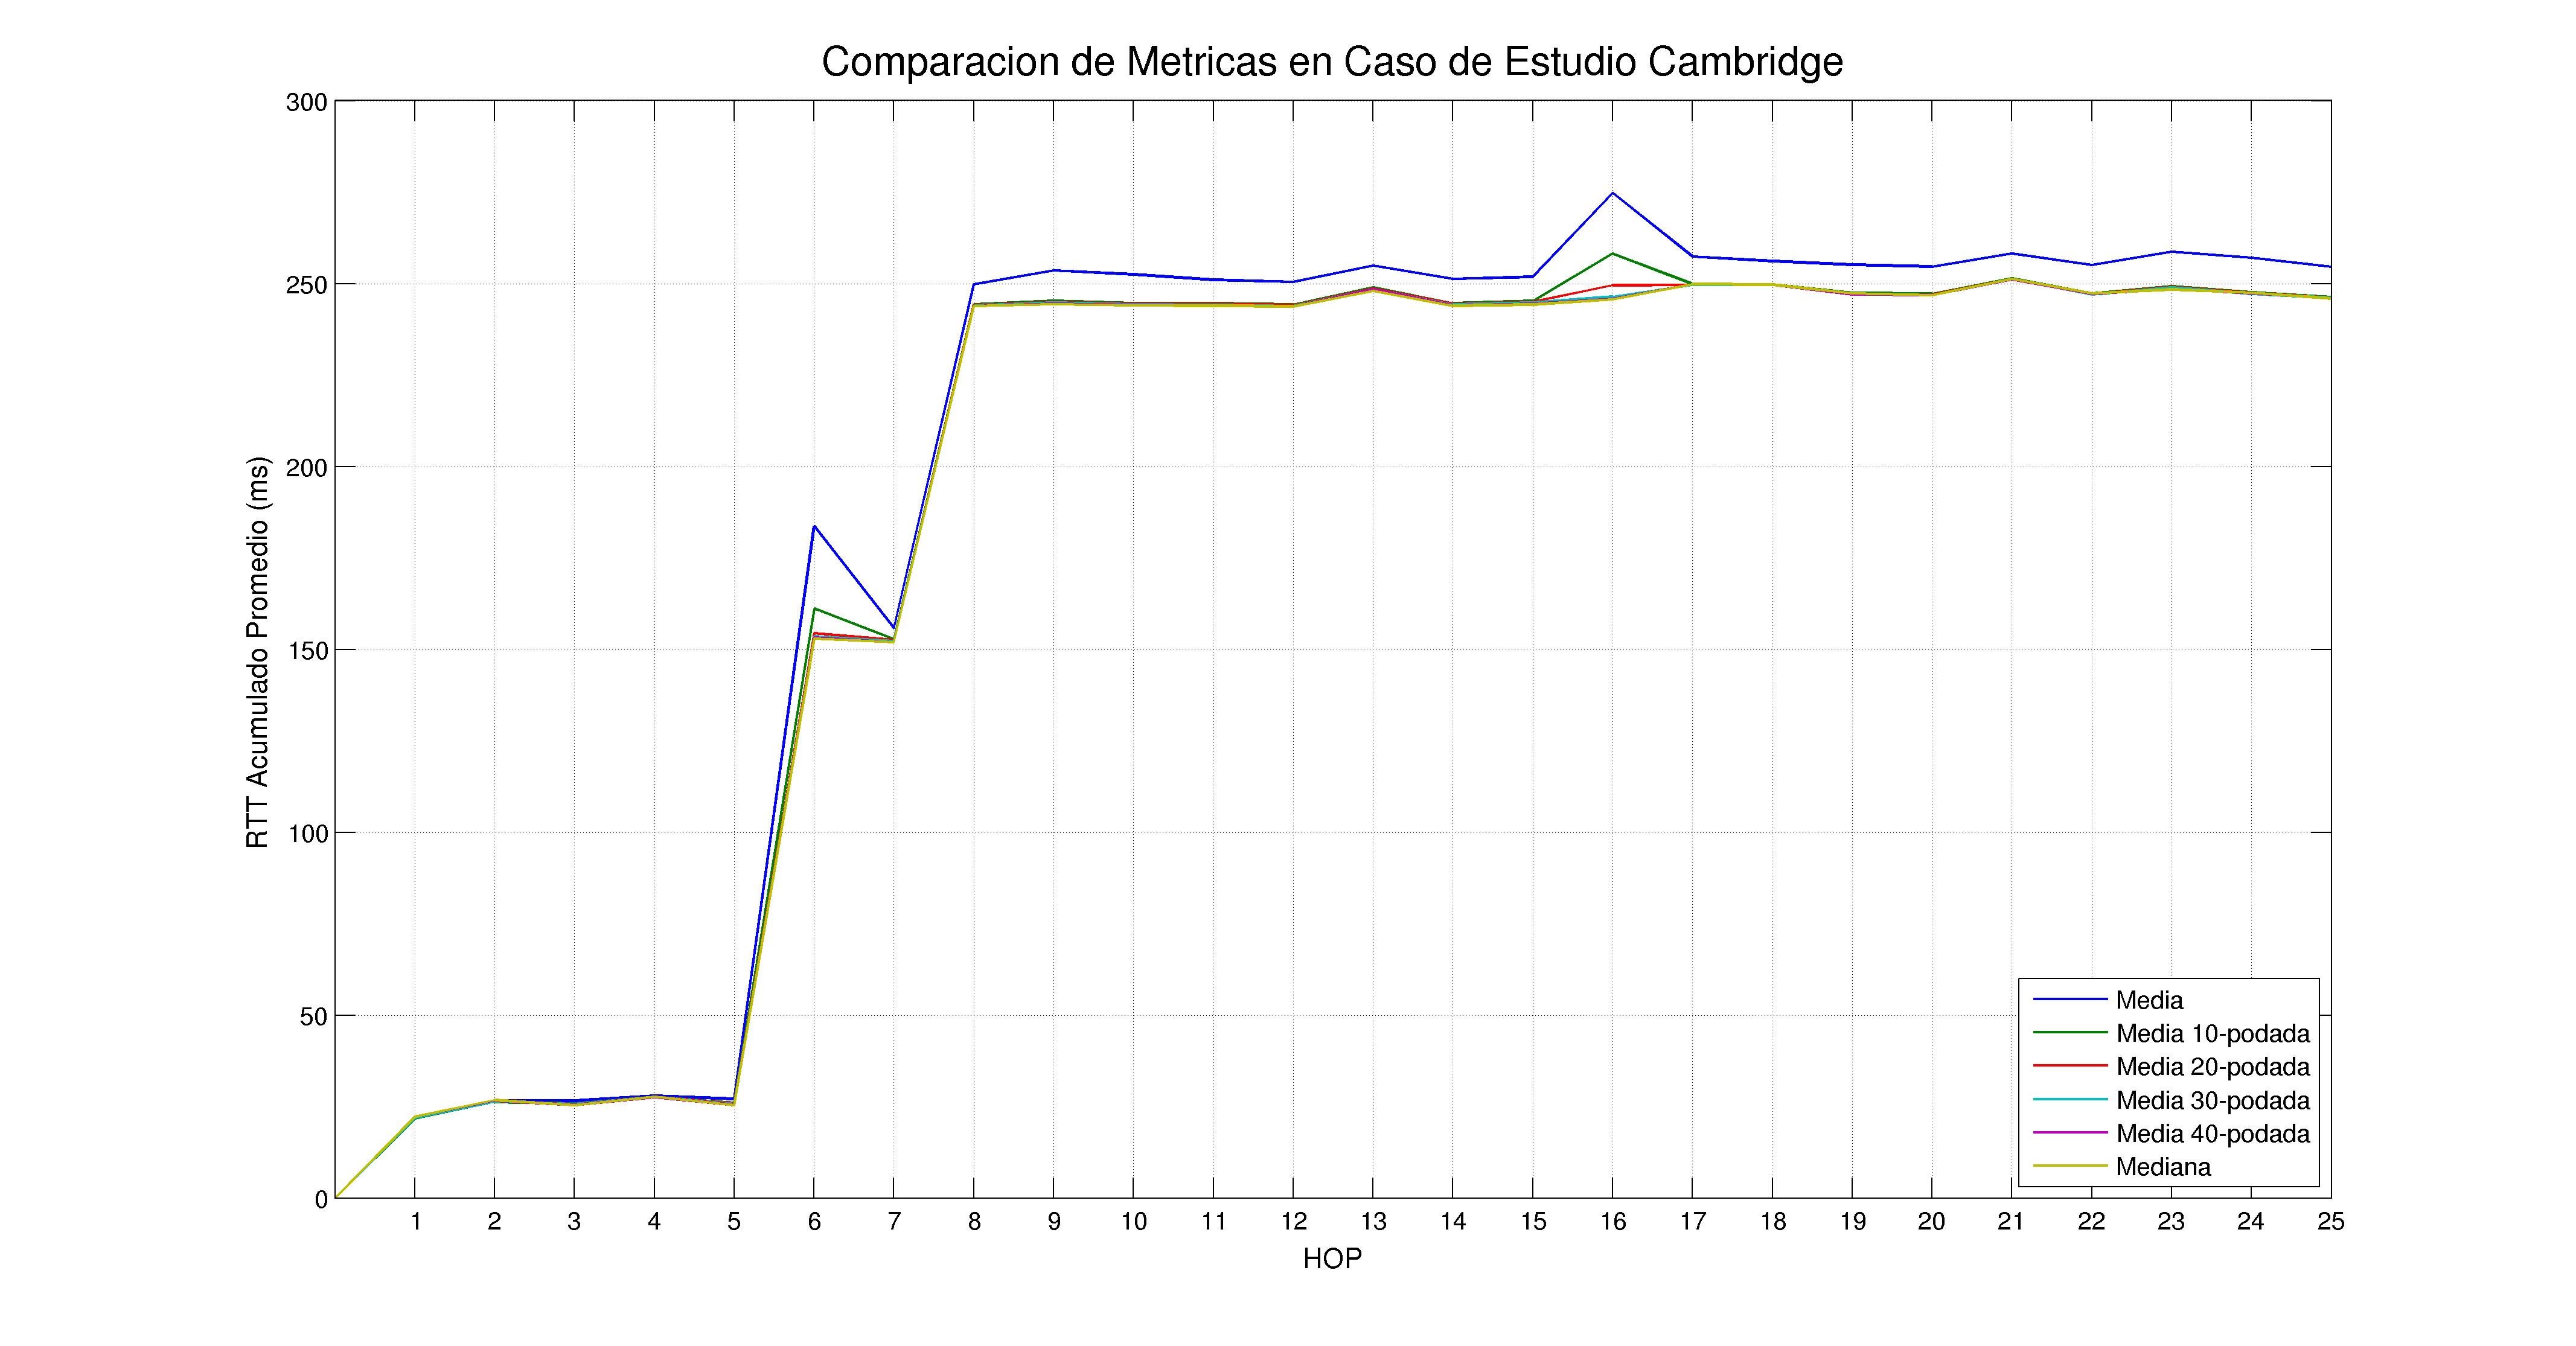
\includegraphics[width=\textwidth]{../resultados/comparacion-metricas-cambridge.png}
 \caption{Comparación de las distintas técnicas para promediar el RTT acumulado, en el caso de estudio de la universidad de Cambridge.}
\end{figure}

\begin{figure}[h!]
 \centering
 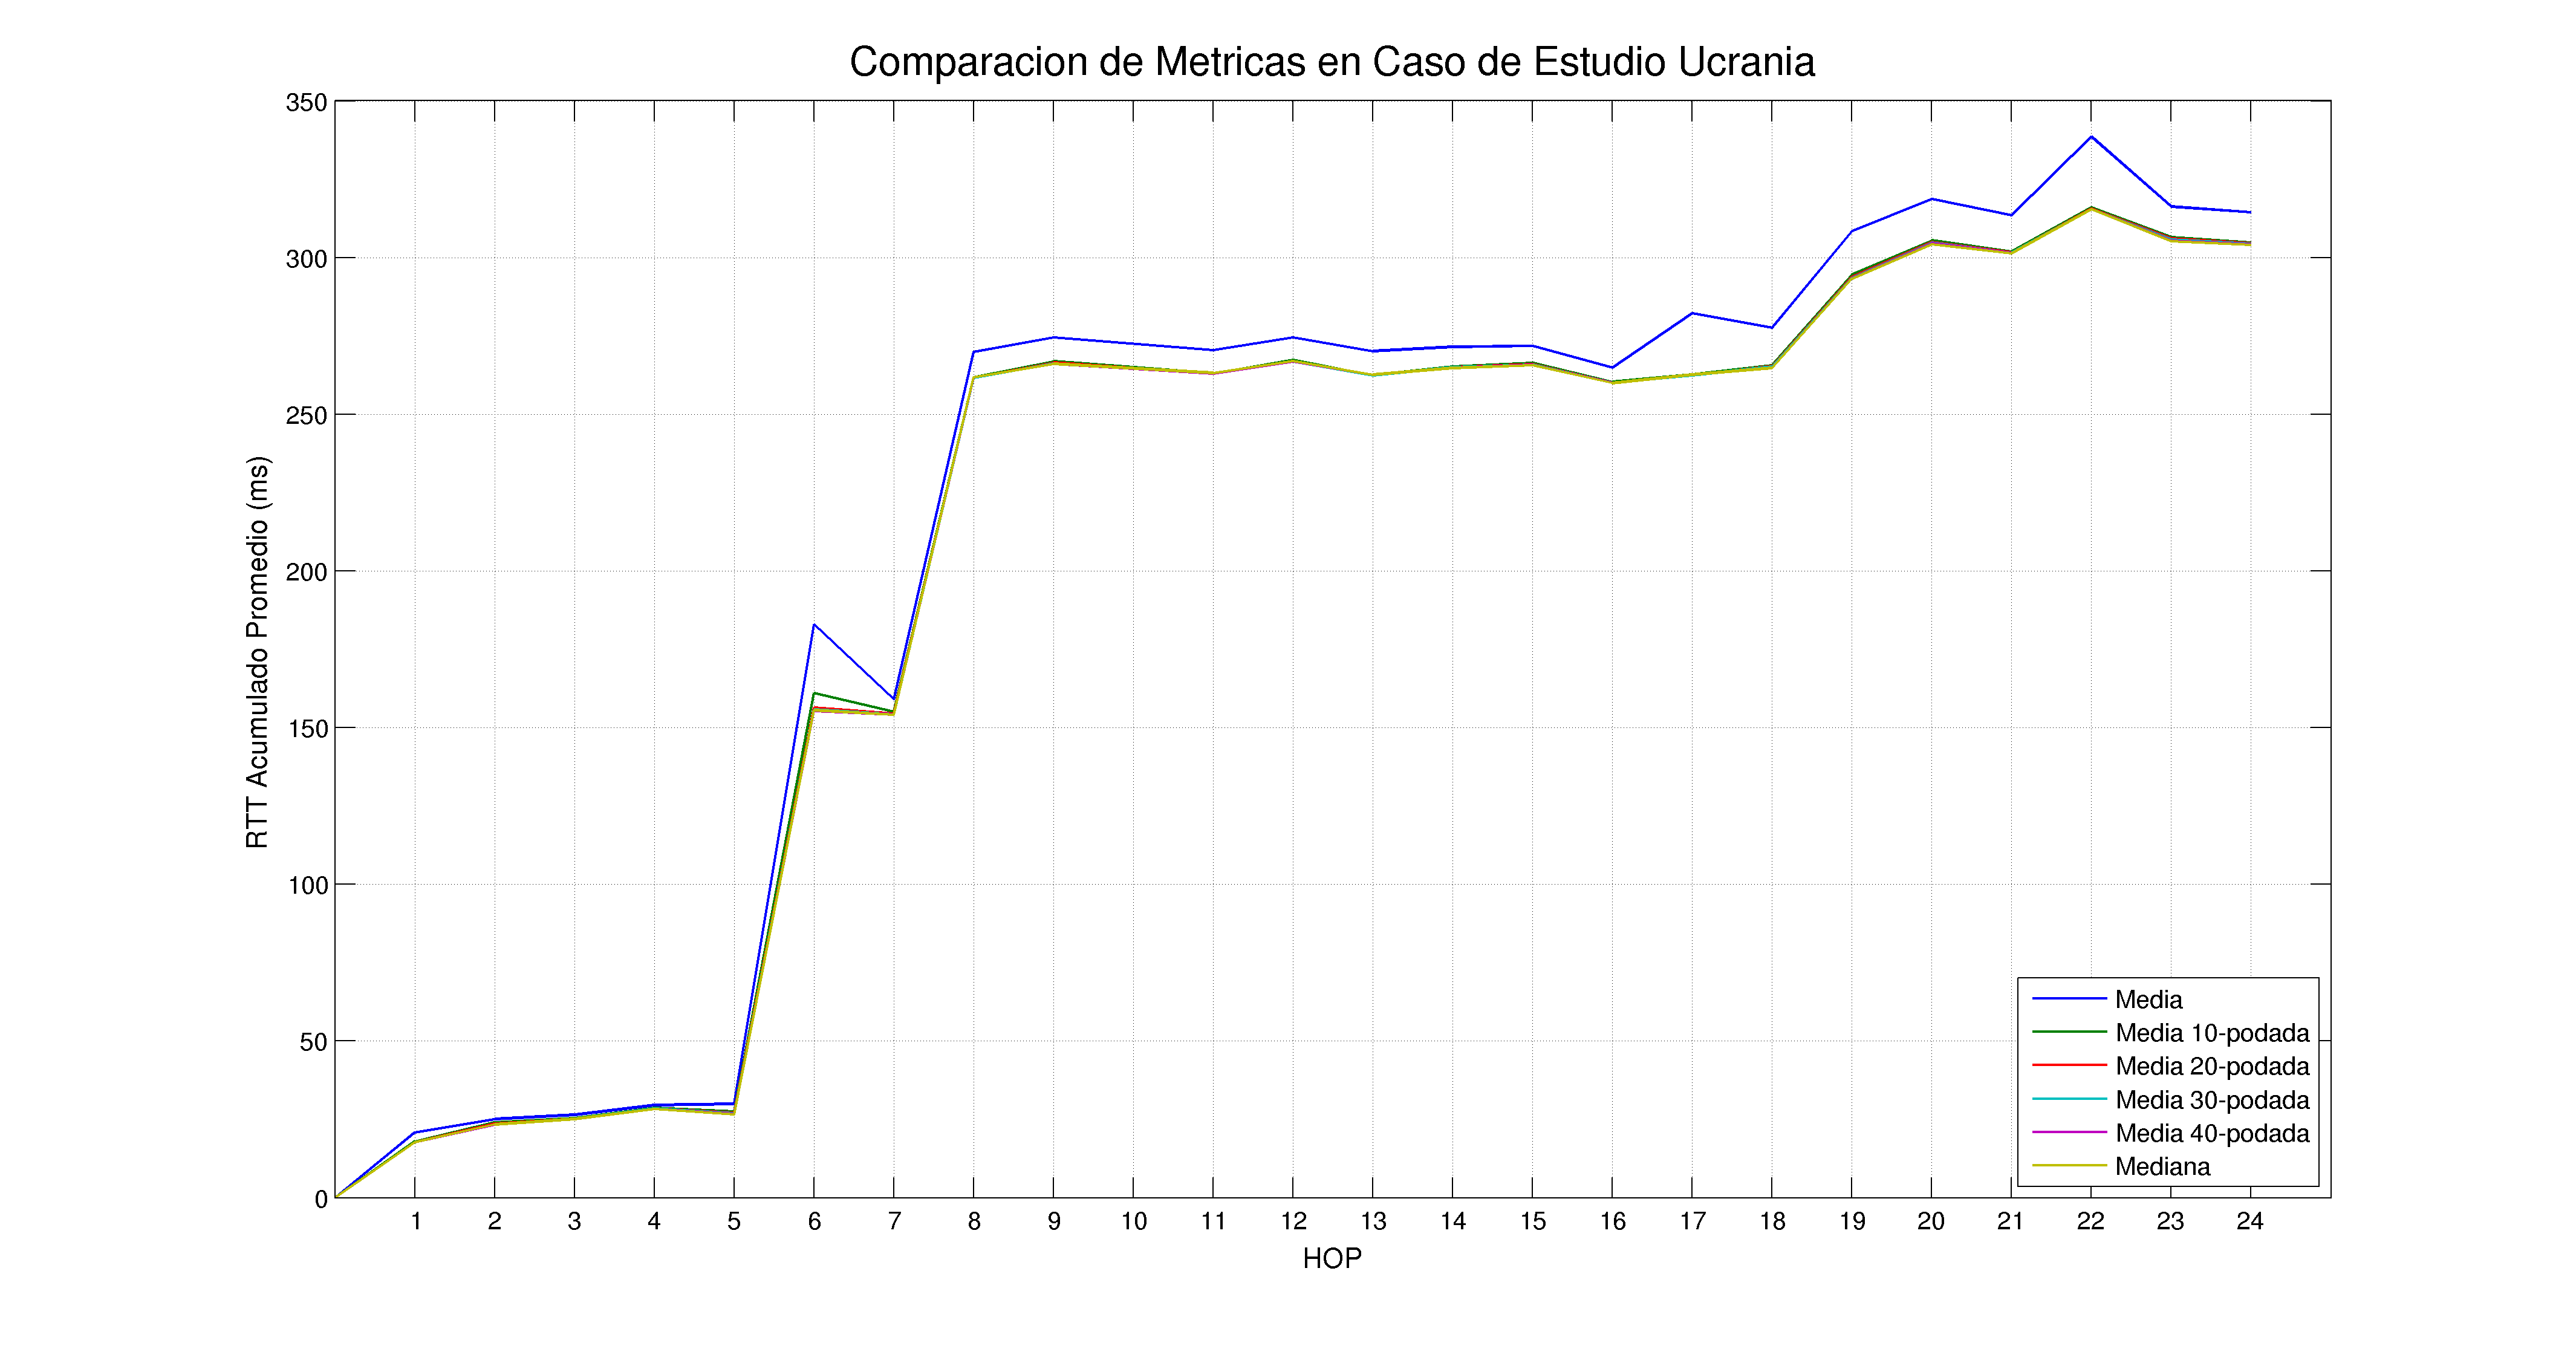
\includegraphics[width=\textwidth]{../resultados/comparacion-metricas-ucrania.png}
 \caption{Comparación de las distintas técnicas para promediar el RTT acumulado, en el caso de estudio de la universidad de Ucrania.}
\end{figure}

\newpage

\begin{figure}[h!]
 \centering
 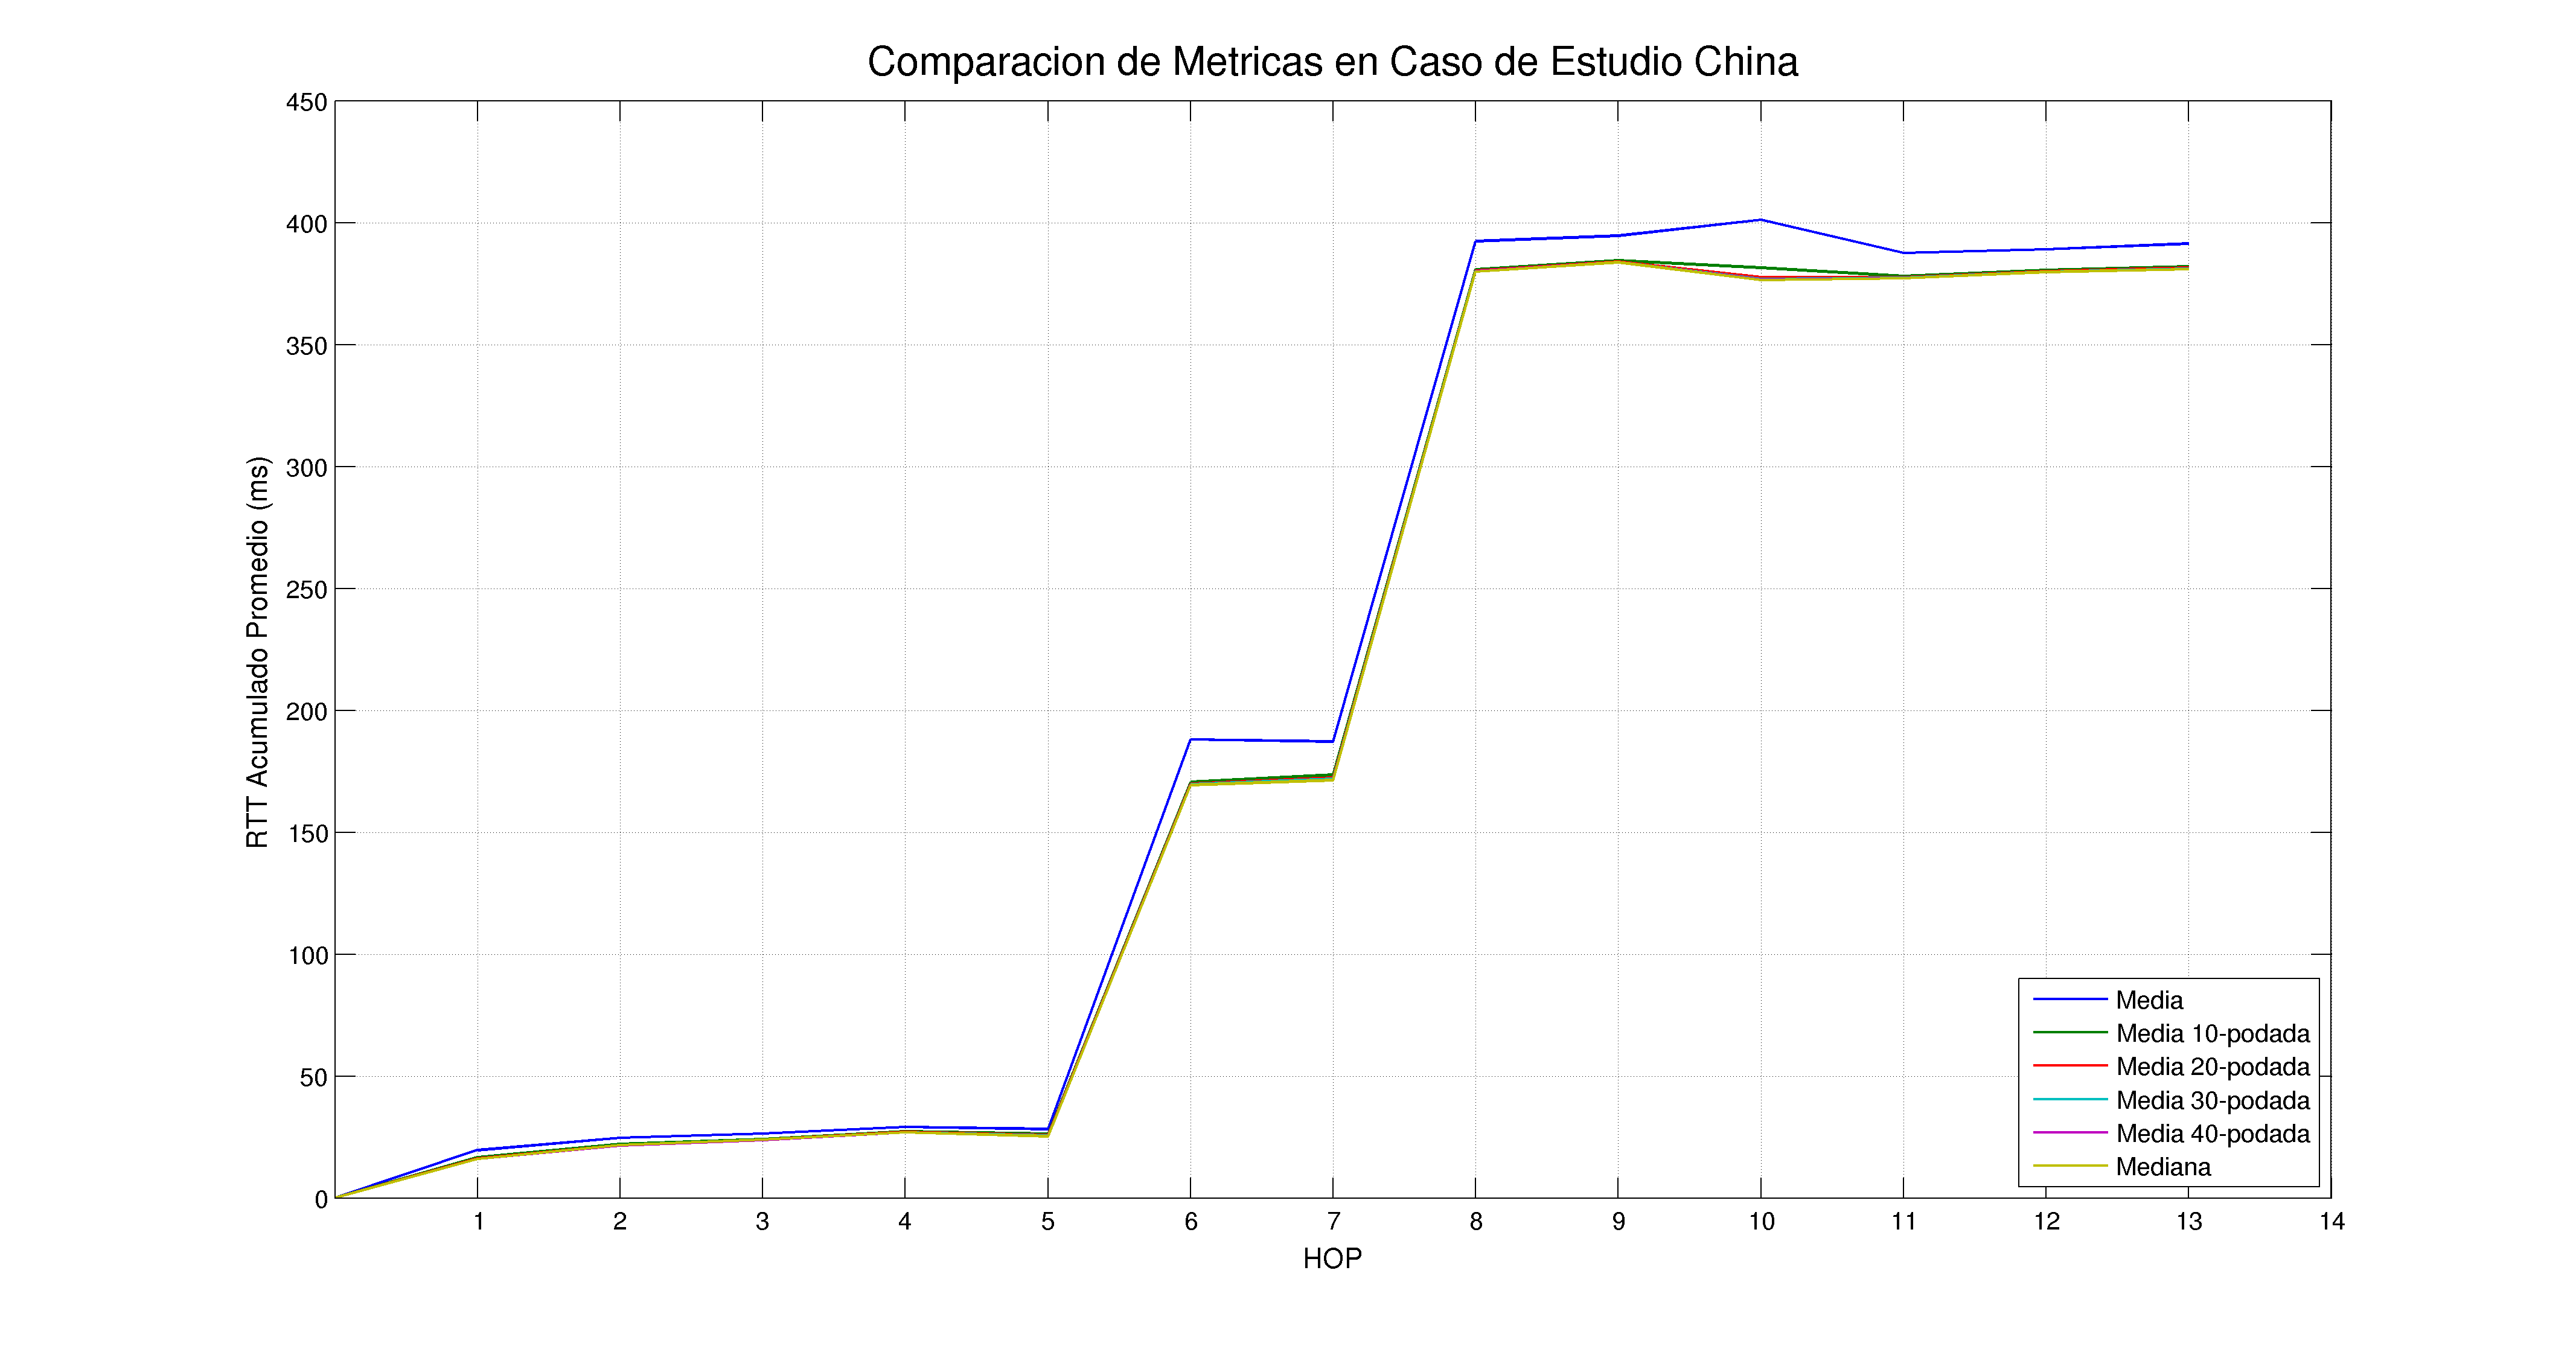
\includegraphics[width=\textwidth]{../resultados/comparacion-metricas-china.png}
 \caption{Comparación de las distintas técnicas para promediar el RTT acumulado, en el caso de estudio de la universidad de China.}
\end{figure}

\newpage

\subsection{Caso de Estudio: Universidad de Cambridge} \label{resultados:cambridge}
\subsubsection{Determinación de Rutas y RTTs de cada salto}
%% Aca decir que se encontró una sola ruta y ponemos directamente la tablita (ttl,ip,icmp,rttAcum,probabilidad,rtt_1_i,rtt_2_i)
%% rtt_1_i vs rtt_2_i

\begin{table}[h!]
  \footnotesize
  \centering
  \begin{tabular}{| r | r | c | r | r | r | r |}
  \hline
  \multicolumn{7}{|c|}{\bf Ruta Más Probable: Cambridge}\\
  \hline\hline
  {\bf\footnotesize TTL} & \multicolumn{1}{|c|}{\bf\footnotesize IP} & \multicolumn{1}{|c|}{\bf\footnotesize ICMP} & {\bf\footnotesize $P(IP|TTL)$} & {\bf\footnotesize $RTT^{acum}_i$ (ms)} & {\bf\footnotesize 1. $RTT_i$ (ms)}& {\bf\footnotesize 2. $RTT_i$ (ms)}\\
  \hline
  \hline
  %%%% TABLA QUE PRODUCE calcular.py :
  \input{../resultados/tabla-cambridge.tab}
  \end{tabular}
  \caption{El camino más utilizado para llegar a Cambridge. Los encabezados utilizan la notación presentada en las secciones \ref{desarrollo:rutas}
  y \ref{desarrollo:rttPorSalto}.}
\end{table}
%% De esta tabla hay que decir: porque rtts acumulados no son estrictamente crecientes, cual es mejor RTT_i segun cual nos da mas informacion,
%% que la ruta es unica porque todas las ips dieron con proba=1, los RTT=0 se corresponden con ips dentro de un mismo sistema autonomo?

\subsubsection{RTTs acumulados y ZRTTs}

\begin{figure}[h!]
 \centering
 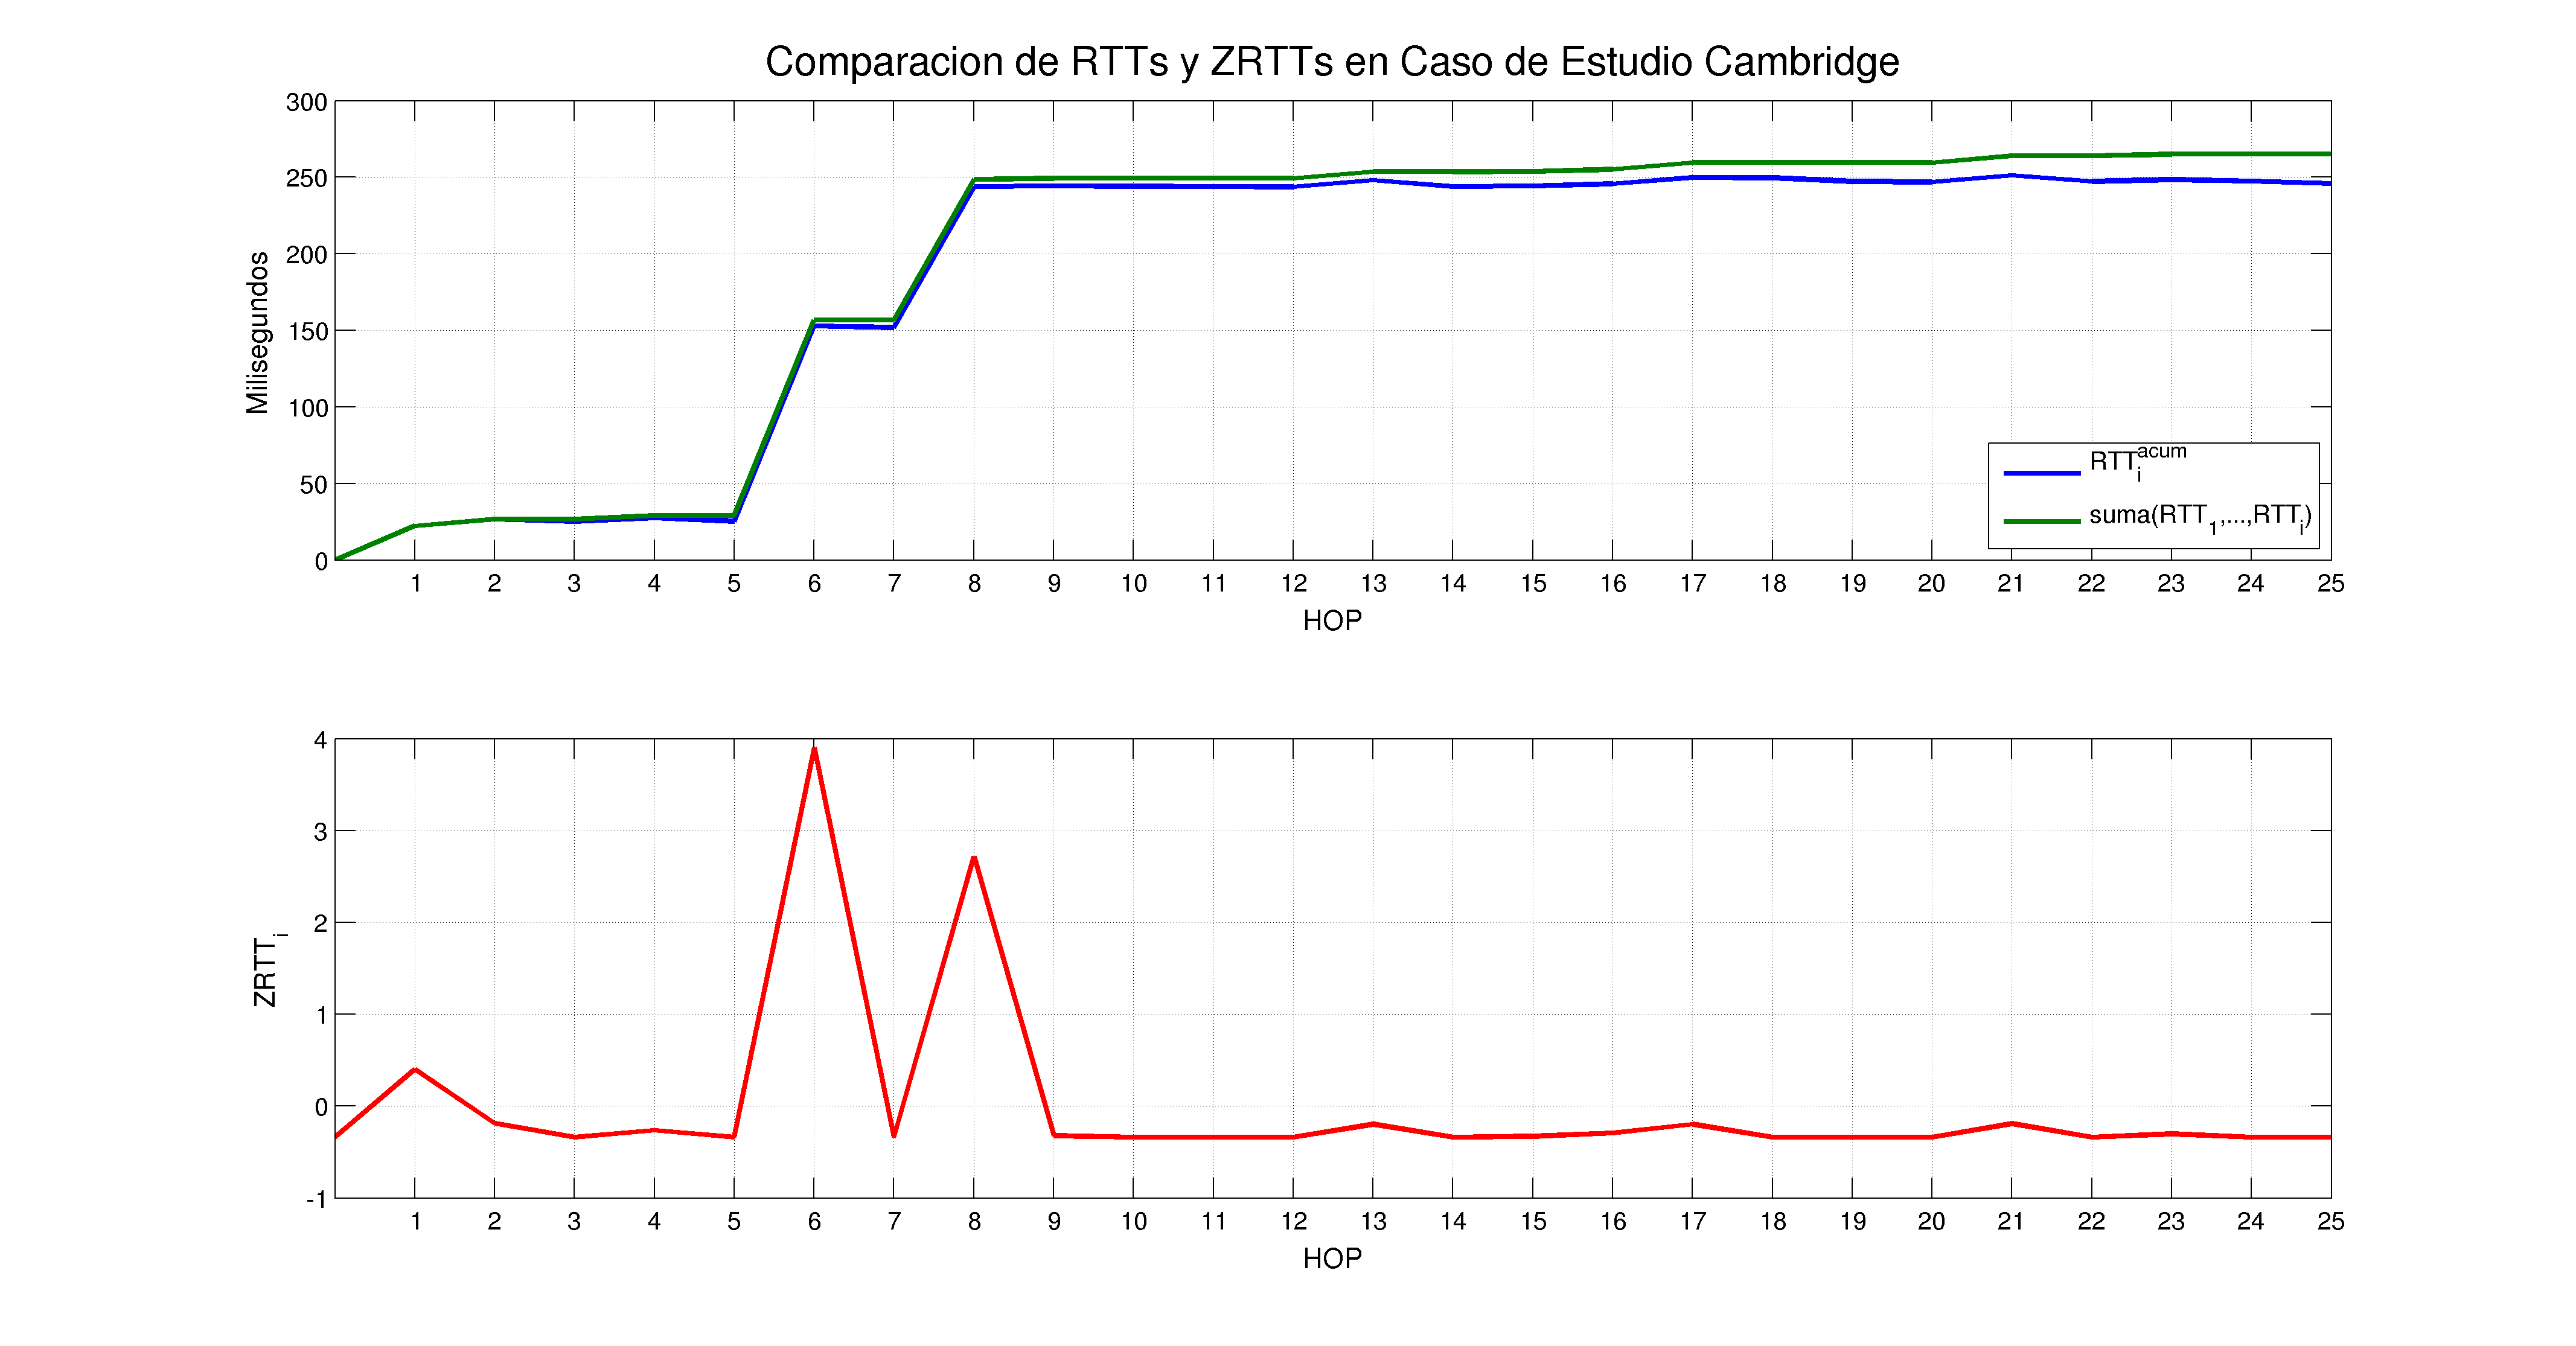
\includegraphics[width=\textwidth]{../resultados/comparacion-zrtts-cambridge.png}
 \caption{Comparación de $RTT^{acum}_i$ con $\sum_{k=1}^{i}RTT_k$ y con $ZRTT_i$.}
 \label{resultados:cambridge:zrtt}
\end{figure}

\newpage

\subsubsection{Geolocalización}

% \begin{figure}[h!]
%  \centering
%  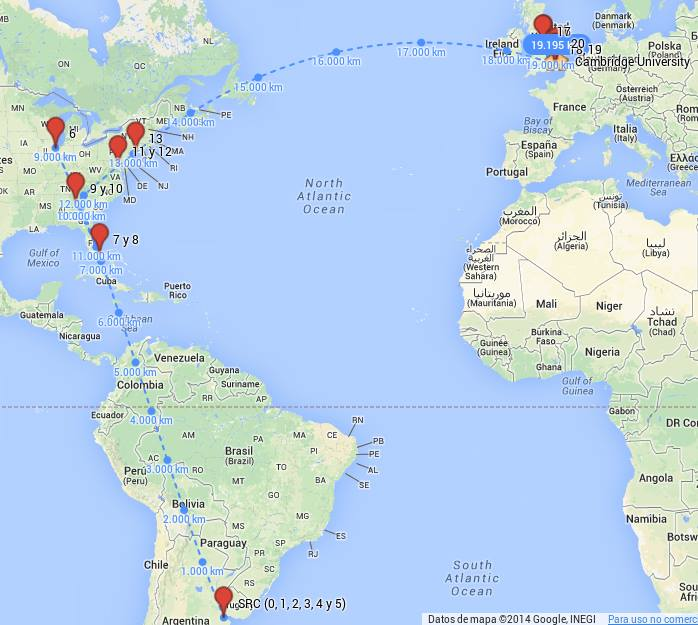
\includegraphics[width=0.5\textwidth]{../resultados/mapa-cambridge-1.jpg}
%  
%  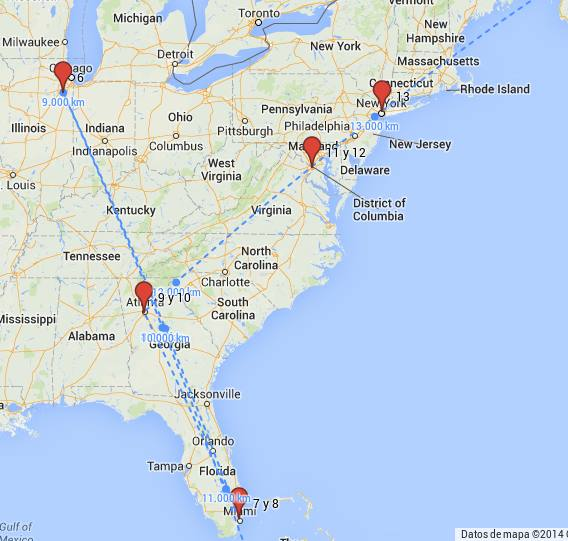
\includegraphics[width=0.45\textwidth]{../resultados/mapa-cambridge-2.jpg}
%  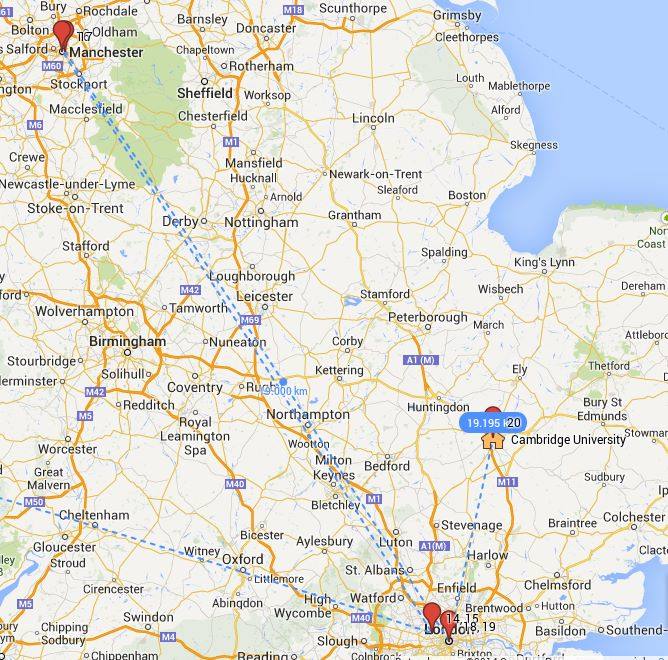
\includegraphics[width=0.45\textwidth]{../resultados/mapa-cambridge-3.jpg}
% 
%  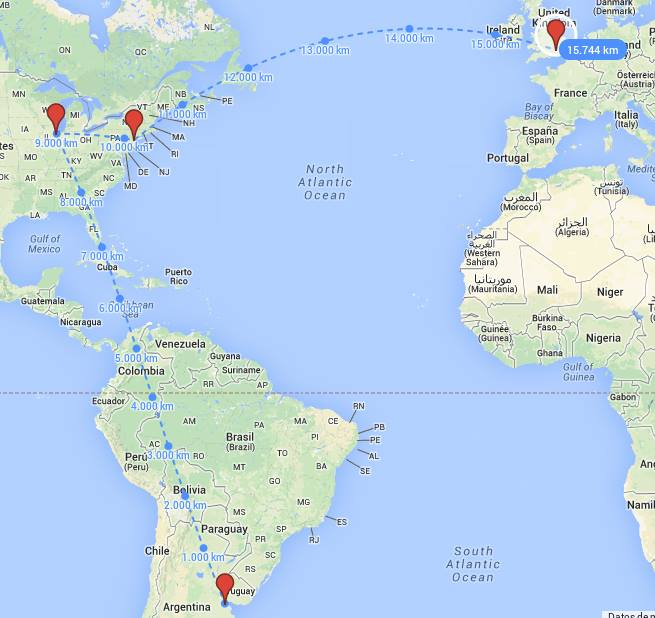
\includegraphics[width=0.5\textwidth]{../resultados/mapa-cambridge-4.jpg}
%  \caption{Mapa}
% \end{figure}
% %% Mapa geolocalizando la ruta
% %% distancias vs rtts, acertamos al enlace submarino con los zscores?
% 
% \newpage

\begin{table}[h!]
  \centering
  \scriptsize
  \begin{adjustwidth}{-1cm}{}
    \begin{tabular}{| r | r | c | c | c |}
    \hline
    \multicolumn{5}{|c|}{\bf Geolocalización: Cambridge}\\
    \hline\hline
    {\bf TTL} & \multicolumn{1}{|c|}{\bf IP} & \multicolumn{1}{|c|}{\bf DNS} & {\bf Ubicación} & {\bf Lat,Lon}\\
    \hline
    \hline
    %%%% TABLA QUE PRODUCE calcular.py :
    \input{../resultados/geoloc-cambridge.tab}
    \end{tabular}
  \end{adjustwidth}
  \caption{\footnotesize Tabla de información de geolocalización del camino más probable para el caso de estudio Cambridge. Observar las celdas resaltadas de arriba hacia abajo: (1) indica que comenzamos en Argentina. (2) dice ``{\tt crossing-argentina}'' lo cual indica que seguimos en Argentina o  cerca. (3) dice ``{\tt ar1.MIA2}'' mientras que las dos anteriores decían ``{\tt ar3.eze1}'' indicando que algo cambió, la red también cambió (ver la IP) y además este salto corresponde al de mayor RTT. (4) El salto para TTL=8 corresponde al segundo salto de mayor RTT, sin embargo de los datos de geolocalización
  no podemos inferir que sea un enlace submarino. (5) Recien en el salto 14 aparece en la DNS la palabra ``{\tt London}'' haciendo referencia
  a Inglaterra (el salto anterior aún decía Estados Unidos en la DNS). (6) Recién en el salto 17 aparece la geolocalización en United Kingdom.}
\end{table}

\begin{figure}[h!]
 \centering
 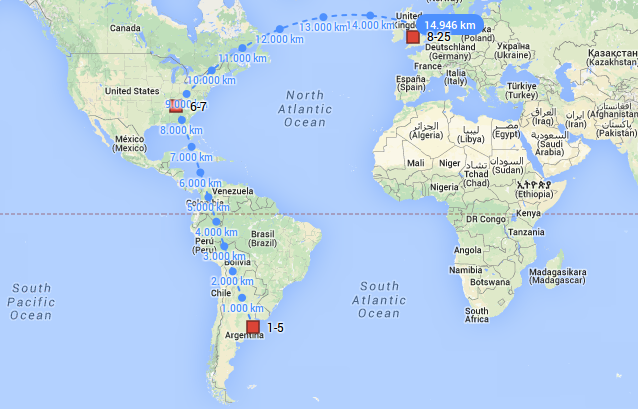
\includegraphics[width=\textwidth, trim = 0 50 0 0, clip]{../resultados/mapa-cambridge.png}
 \caption{Mapa generado utilizando los datos de la tabla anterior y los valores de $RRT_i$ empíricos.}
\end{figure}

\newpage

\subsection{Caso de Estudio: Universidad de Ucrania} \label{resultados:ucrania}

\subsubsection{Determinación de Rutas y RTTs de cada salto}
%% Aca decir que se encontró una sola ruta y ponemos directamente la tablita (ttl,ip,icmp,rttAcum,probabilidad,rtt_1_i,rtt_2_i)
%% rtt_1_i vs rtt_2_i

% \begin{table}[h!]
%   \centering
%   \footnotesize
%   \begin{tabular}{| r || r | c | r || r | c | r || r | c | r |}
%   \hline
%   \multicolumn{10}{|c|}{\bf Rutas Más Probables}\\
%   \hline\hline
%   {\bf\footnotesize TTL} & \multicolumn{1}{|c|}{\bf\footnotesize IP1} & \multicolumn{1}{|c|}{\bf\footnotesize ICMP1} & {\bf\footnotesize P1}  & \multicolumn{1}{|c|}{\bf\footnotesize IP2} & \multicolumn{1}{|c|}{\bf\footnotesize ICMP2} & {\bf\footnotesize P2} & \multicolumn{1}{|c|}{\bf\footnotesize IP3} & \multicolumn{1}{|c|}{\bf\footnotesize ICMP3} & {\bf\footnotesize P3}\\
%   \hline
%   \hline
%   %%%% TABLA QUE PRODUCE calcular.py :
%   \input{../resultados/kiev_caminos_latex.txt}
%   \end{tabular}
%   \caption{Los caminos más utilizado para llegar a Ucrania. Los encabezados utilizan la notación presentada en las secciones \ref{desarrollo:rutas}
%   y \ref{desarrollo:rttPorSalto}.}
% \end{table}

\begin{table}[h!]
  \centering
  \footnotesize
  \begin{tabular}{| r || r | c | r || r | c | r |}
  \hline
  \multicolumn{7}{|c|}{\bf Rutas Encontradas: Ucrania}\\
  \hline\hline
  {\bf\footnotesize TTL} & \multicolumn{1}{|c|}{\bf\footnotesize IP1} & \multicolumn{1}{|c|}{\bf\footnotesize ICMP1} & {\bf\footnotesize P1}  & \multicolumn{1}{|c|}{\bf\footnotesize IP2} & \multicolumn{1}{|c|}{\bf\footnotesize ICMP2} & {\bf\footnotesize P2} \\
  \hline
  \hline
  %%%% TABLA QUE PRODUCE calcular.py :
  \input{../resultados/kiev_caminos_latex.txt}
  \end{tabular}
  \label{resultados:Ucrania:caminos}
  \caption{Las rutas encontradas para llegar a Ucrania. La numeración en los encabezados indica el número de ruta, ordenadas por probabilidad.}
\end{table}

\newpage
\begin{table}[h!]
  \centering
  \footnotesize
  \begin{tabular}{| r | r | c | r | r | r | r |}
  \hline
  \multicolumn{7}{|c|}{\bf Ruta Más Probable: Ucrania}\\
  \hline\hline
  {\bf\footnotesize TTL} & \multicolumn{1}{|c|}{\bf\footnotesize IP} & \multicolumn{1}{|c|}{\bf\footnotesize ICMP} & {\bf\footnotesize $P(IP|TTL)$} & {\bf\footnotesize $RTT^{acum}_i$ (ms)} & {\bf\footnotesize 1. $RTT_i$ (ms)}& {\bf\footnotesize 2. $RTT_i$ (ms)}\\
  \hline
  \hline
  %%%% TABLA QUE PRODUCE calcular.py :
  \input{../resultados/kiev_caminoMasProbable_latex.txt}
  \end{tabular}
  \label{resultados:Ucrania:camino}
  \caption{El camino más utilizado para llegar a Ucrania. Los encabezados utilizan la notación presentada en las secciones \ref{desarrollo:rutas}
  y \ref{desarrollo:rttPorSalto}.}
\end{table}
%% De esta tabla hay que decir: porque rtts acumulados no son estrictamente crecientes, cual es mejor RTT_i segun cual nos da mas informacion,
%% que la ruta es unica porque todas las ips dieron con proba=1, los RTT=0 se corresponden con ips dentro de un mismo sistema autonomo?


\subsubsection{RTTs acumulados y ZRTTs}

\begin{figure}[h!]
 \centering
 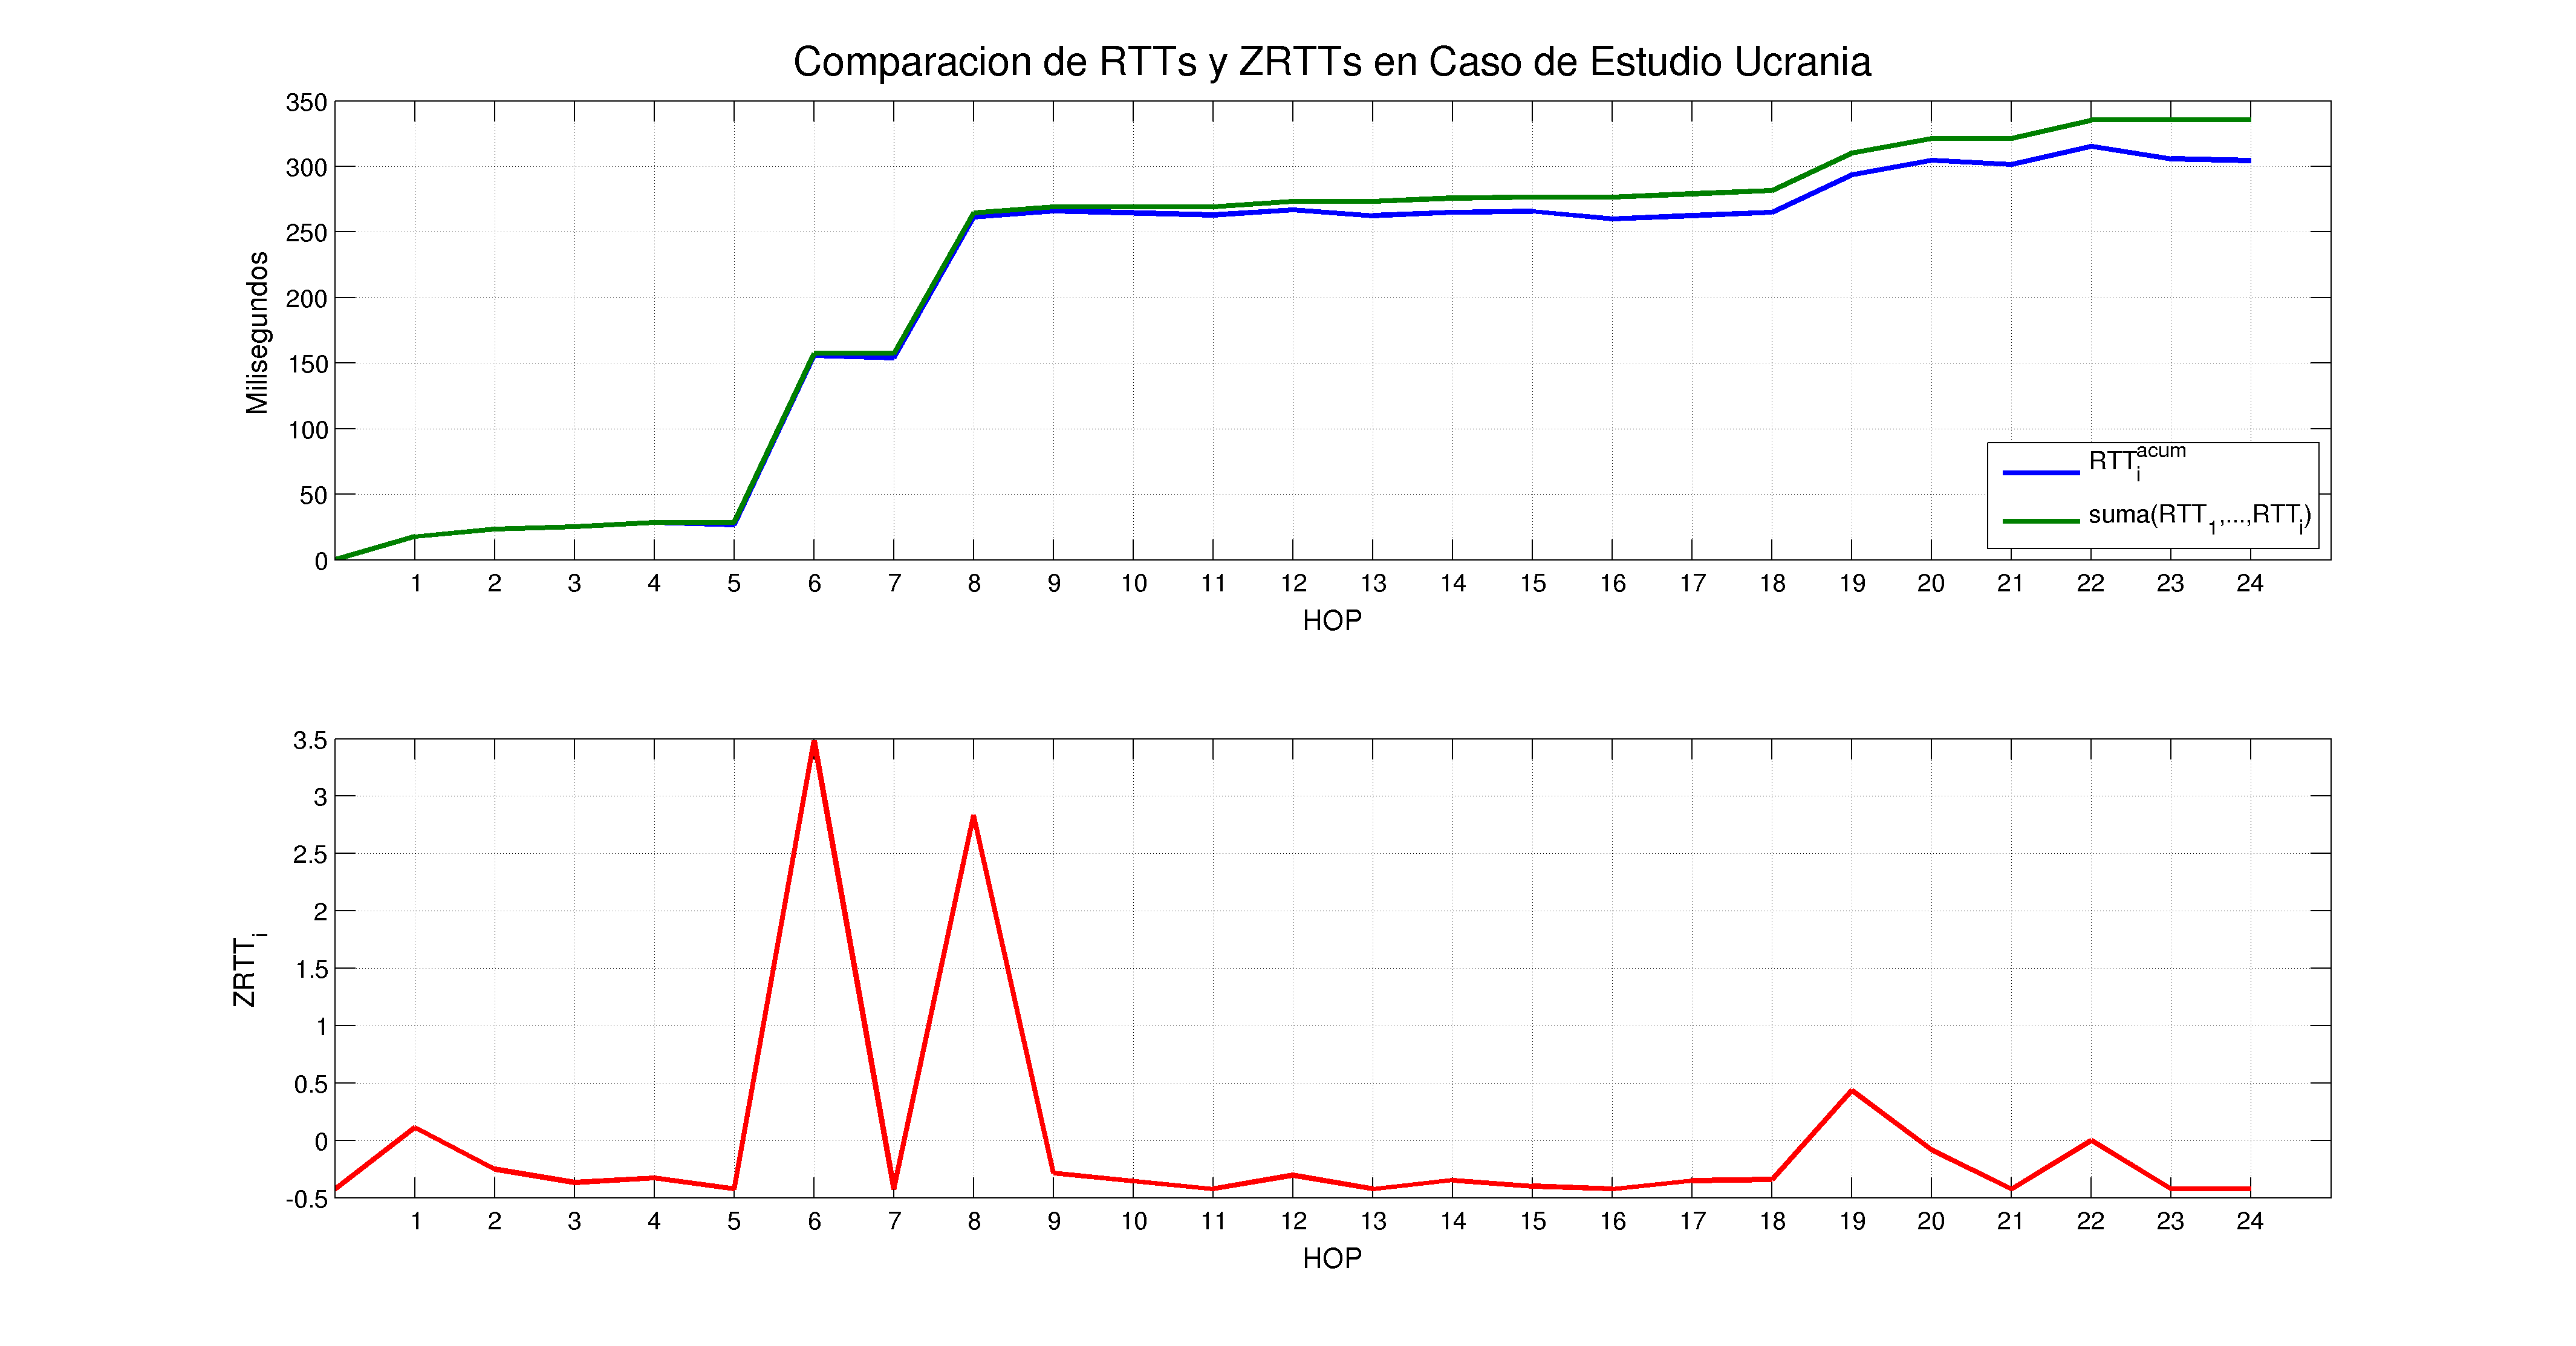
\includegraphics[width=\textwidth]{../resultados/comparacion-zrtts-ucrania.png}
 \caption{Comparación de $RTT^{acum}_i$ con $\sum_{k=1}^{i}RTT_k$ y con $ZRTT_i$.}
 \label{resultados:Ucrania:zrtt}
\end{figure}


\newpage
\subsubsection{Geolocalización}

\begin{table}[h!]
  \centering
  \scriptsize
  \begin{adjustwidth}{-0.6cm}{}
    \begin{tabular}{| r | r | c | c | c |}
    \hline
    \multicolumn{5}{|c|}{\bf Geolocalización: Ucrania}\\
    \hline\hline
    {\bf TTL} & \multicolumn{1}{c|}{\bf IP} & \multicolumn{1}{c|}{\bf DNS} & {\bf Ubicación} & {\bf Lat,Lon}\\
    \hline
    \hline
    %%%% TABLA QUE PRODUCE calcular.py :
    \input{../resultados/geoloc-ucrania.tab}
    \label{resultados:ucrania:geolocalizar}
    \end{tabular}
  \end{adjustwidth}
  \caption{\footnotesize Tabla de información de geolocalización del camino más probable para el caso de estudio Ucrania. Observar las celdas resaltadas de arriba hacia abajo: (1) indica que comenzamos en Argentina. (2) dice ``{\tt crossing-argentina}'' lo cual indica que seguimos en Argentina o  cerca. (3) dice ``{\tt ar1.MIA2}'' mientras que las dos anteriores decían ``{\tt ar3.eze1}'' indicando que algo cambió, la red también cambió (ver la IP) y además este salto corresponde al de mayor RTT. (4) El salto para TTL=8 corresponde al segundo salto de mayor RTT, sin embargo de los datos de geolocalización
  no podemos inferir que sea un enlace submarino. (5) Recien en el salto 14 aparece en la DNS la palabra ``{\tt Paris}'' haciendo referencia
  a Francia (el salto anterior aún decía Estados Unidos en la DNS). (6) En el salto 15 aparece en la DNS la palabra ``{\tt Frankfurt}'' haciendo
  referencia a Alemania (observar que aún la geolocalización indica Estados Unidos). (7) Por primera vez la geolocalización cambió de continente.
  (8) El salto 19 sobresale en cuanto al valor de RTT y además se corresponde con un salto intercontinental (no necesariamente submarino) de Europa
  a Asia, además observar que la DNS dice ``{\tt kiev}'' con lo cual podría ser que ya hemos llegado a Ucrania y la geolocalización es errónea. (9) La geolocalización indica Ucrania.}
\end{table}

\begin{figure}[h!]
 \centering
 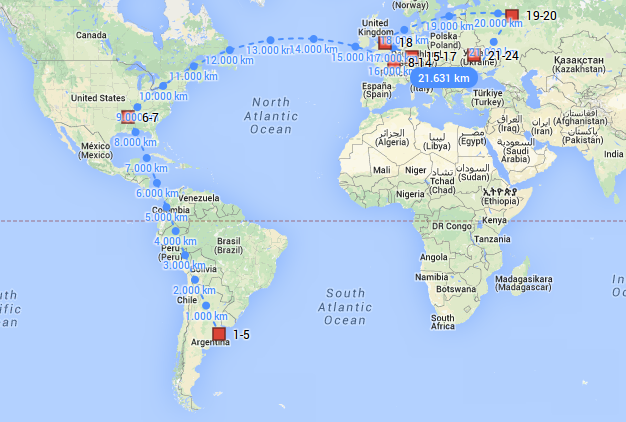
\includegraphics[width=\textwidth, trim = 0 60 0 0, clip]{../resultados/mapa-ucrania.png}
 \caption{Mapa generado utilizando los datos de la tabla anterior y los valores de $RRT_i$ empíricos.}
\end{figure}


\newpage
\subsection{Caso de Estudio: Universidad de China} \label{resultados:china}

\subsubsection{Determinación de Rutas y RTTs de cada salto}
%% Aca decir que se encontró una sola ruta y ponemos directamente la tablita (ttl,ip,icmp,rttAcum,probabilidad,rtt_1_i,rtt_2_i)
%% rtt_1_i vs rtt_2_i

\begin{table}[h!]
  \centering
  \footnotesize
  \begin{tabular}{| r | r | c | r | r | r | r |}
  \hline
  \multicolumn{7}{|c|}{\bf Ruta Más Probable: China}\\
  \hline\hline
  {\bf\footnotesize TTL} & \multicolumn{1}{|c|}{\bf\footnotesize IP} & \multicolumn{1}{|c|}{\bf\footnotesize ICMP} & {\bf\footnotesize $P(IP|TTL)$} & {\bf\footnotesize $RTT^{acum}_i$ (ms)} & {\bf\footnotesize 1. $RTT_i$ (ms)}& {\bf\footnotesize 2. $RTT_i$ (ms)}\\
  \hline
  \hline
  %%%% TABLA QUE PRODUCE calcular.py :
  \input{../resultados/tabla-china.tab}
  \end{tabular}
  \caption{El camino más utilizado para llegar a China. Los encabezados utilizan la notación presentada en las secciones \ref{desarrollo:rutas}
  y \ref{desarrollo:rttPorSalto}.}
  \label{resultados:china:rtts}
\end{table}
%% De esta tabla hay que decir: porque rtts acumulados no son estrictamente crecientes, cual es mejor RTT_i segun cual nos da mas informacion,
%% que la ruta es unica porque todas las ips dieron con proba=1, los RTT=0 se corresponden con ips dentro de un mismo sistema autonomo?


\subsubsection{RTTs acumulados y ZRTTs}

\begin{figure}[h!]
 \centering
 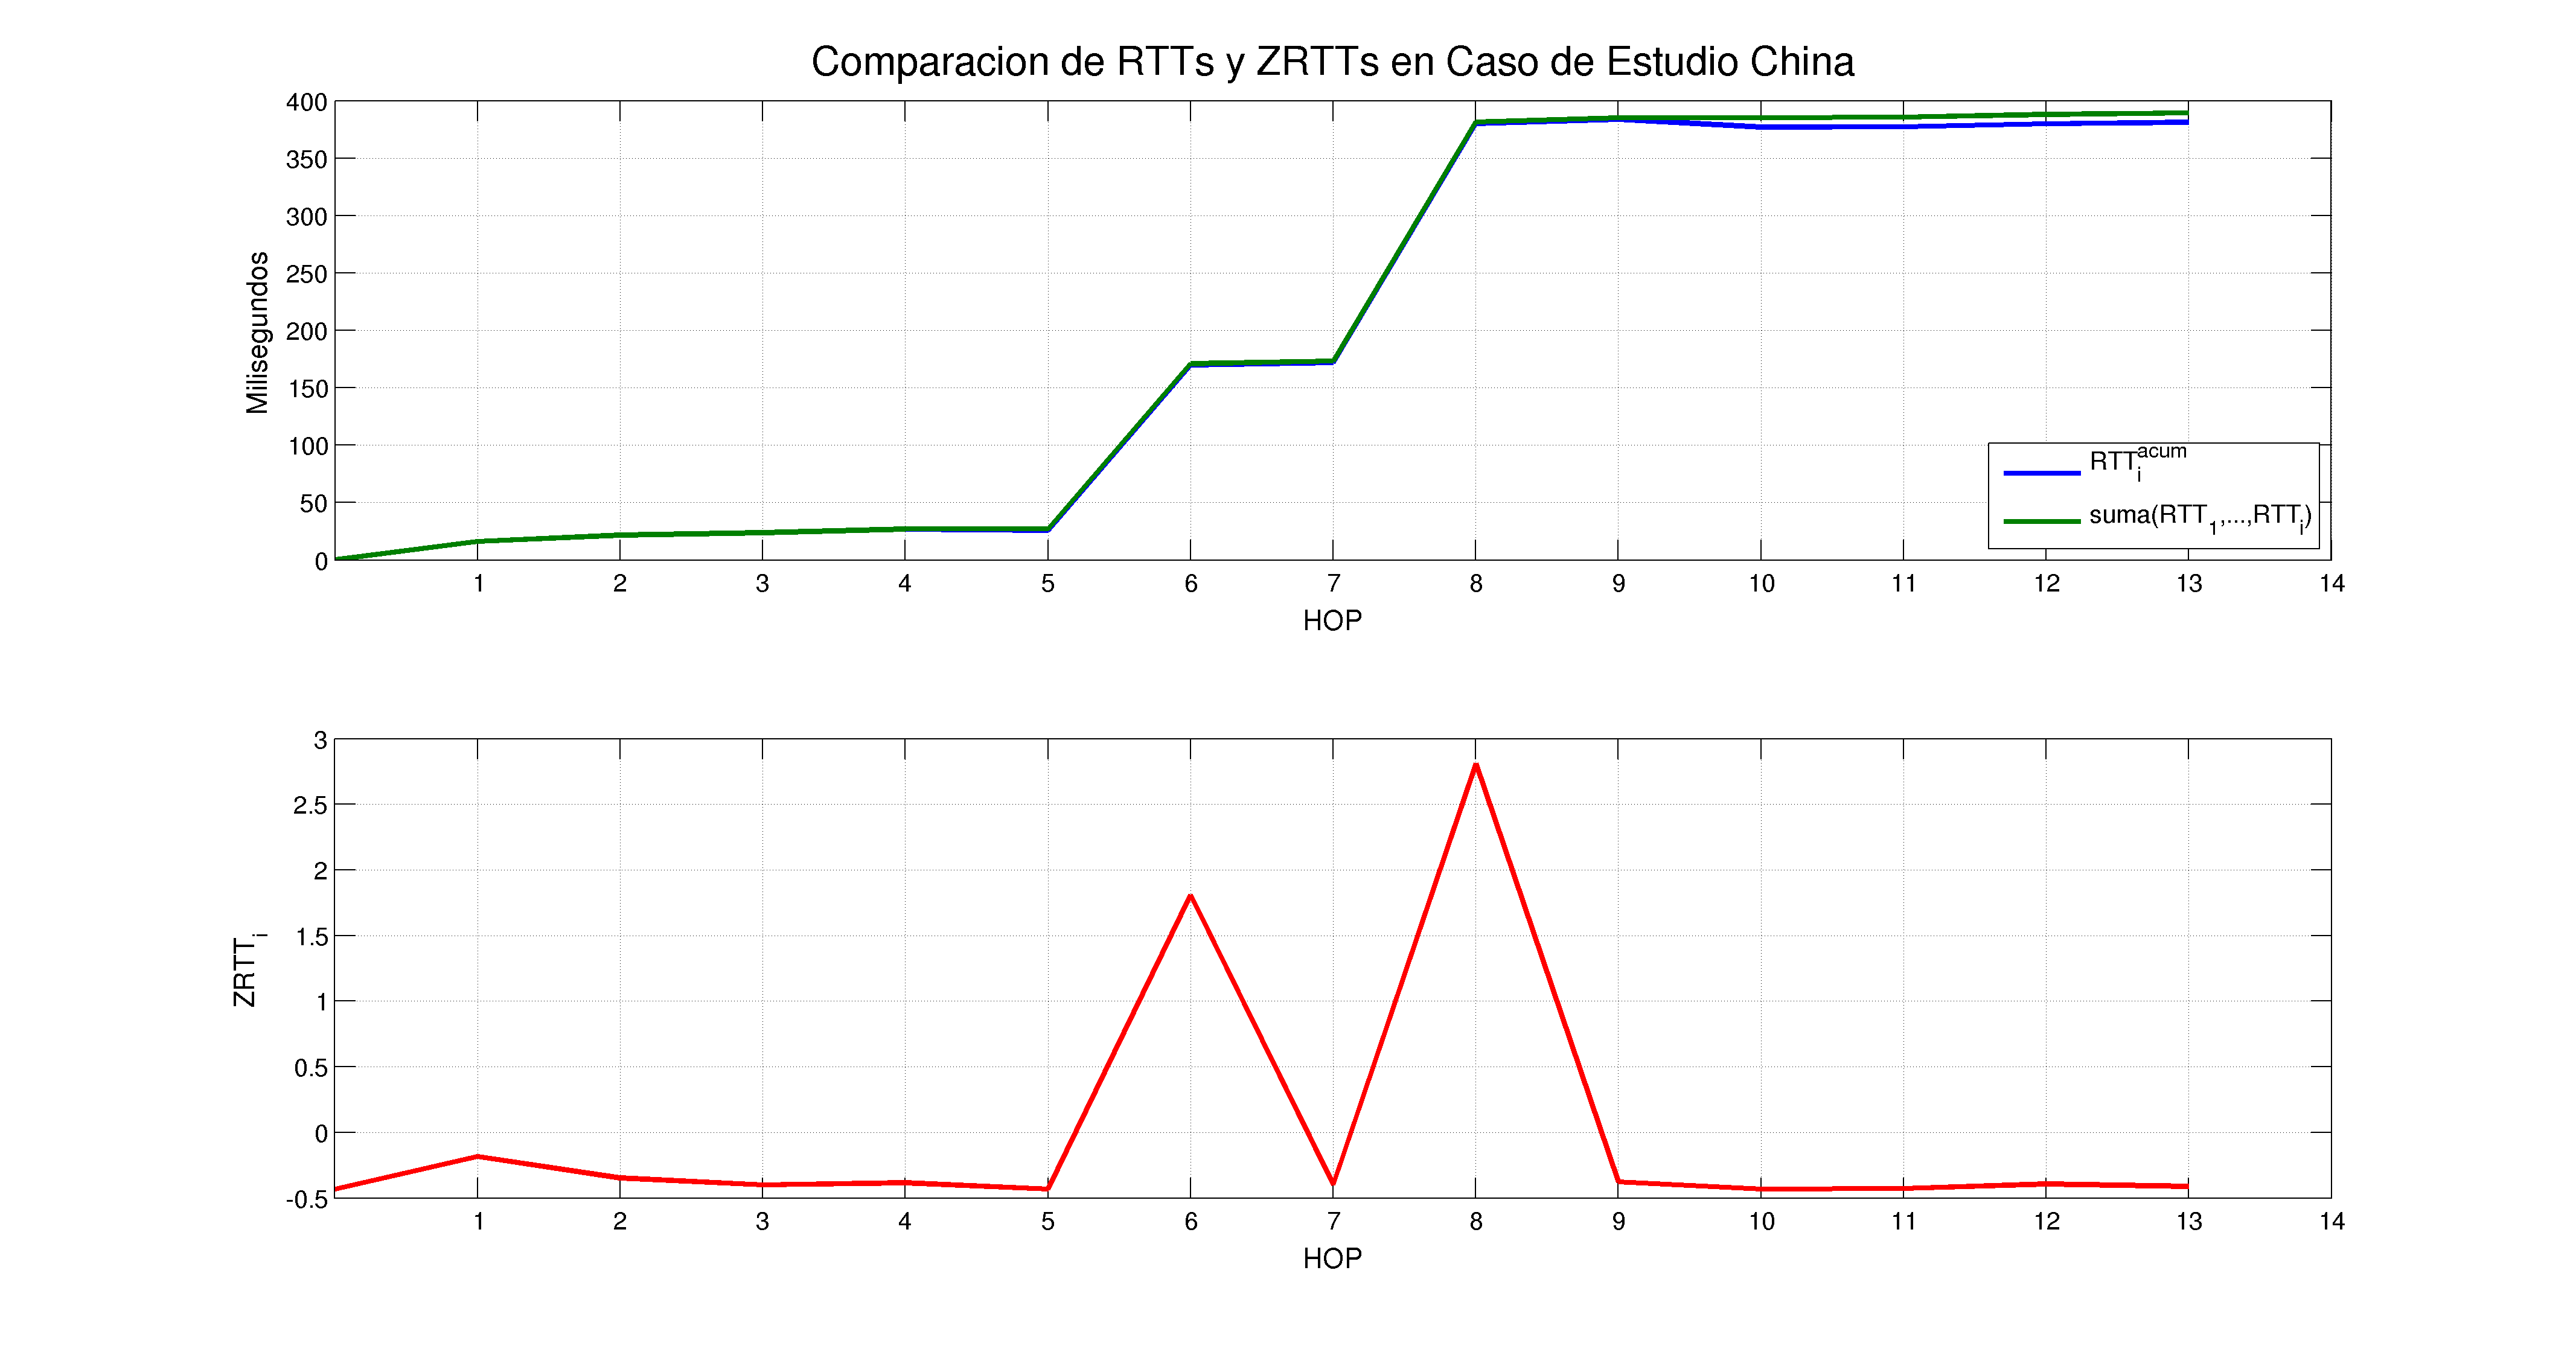
\includegraphics[width=\textwidth]{../resultados/comparacion-zrtts-china.png}
 \caption{Comparación de $RTT^{acum}_i$ con $\sum_{k=1}^{i}RTT_k$ y con $ZRTT_i$.}
 \label{resultados:china:zrtt}
\end{figure}


\newpage
\subsubsection{Geolocalización}

\begin{table}[h!]
  \centering
  \scriptsize
  \begin{adjustwidth}{-0.5cm}{}
    \begin{tabular}{| r | r | c | c | c |}
    \hline
    \multicolumn{5}{|c|}{\bf Geolocalización: China}\\
    \hline\hline
    {\bf TTL} & \multicolumn{1}{|c|}{\bf IP} & \multicolumn{1}{|c|}{\bf DNS} & {\bf Ubicación} & {\bf Lat,Lon}\\
    \hline
    \hline
    %%%% TABLA QUE PRODUCE calcular.py :
    \input{../resultados/geoloc-china.tab}
    \end{tabular}
  \end{adjustwidth}
  \caption{\footnotesize Tabla de información de geolocalización del camino más probable para el caso de estudio China. Observar las celdas resaltadas de arriba hacia abajo: (1) indica que comenzamos en Argentina. (2) dice ``{\tt crossing-argentina}'' lo cual indica que seguimos en Argentina o  cerca. (3) dice ``{\tt ar4.LAX1}'' mientras que las dos anteriores decían ``{\tt ar3.eze1}'' indicando que algo cambió, la red también cambió (ver la IP) y además este salto corresponde al de mayor RTT. (4) Este es el segundo salto de mayor RTT, observar que dice ``{\tt hkg05}'', lo cual se puede interpretar
  como una sigla para ``Hong Kong'', además es razonable creer esto porque todos los saltos restantes tienen ubicación en esa ciudad.}
\end{table}

\begin{figure}[h!]
 \centering
 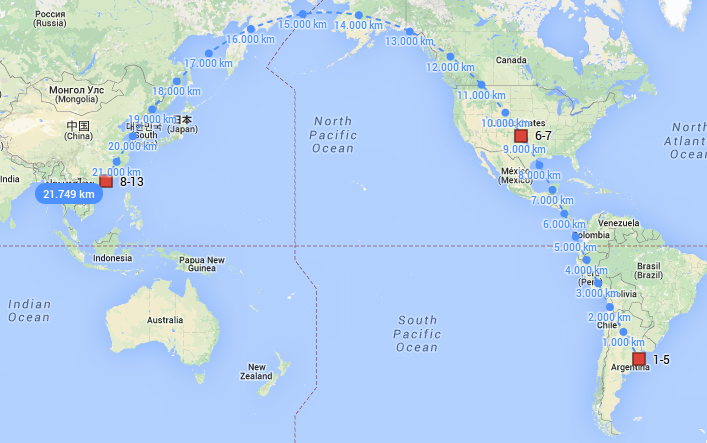
\includegraphics[width=\textwidth]{../resultados/mapa-china.png}
 \caption{Mapa generado utilizando los datos de la tabla anterior y los valores de $RRT_i$ empíricos.}
\end{figure}
% Mapa geolocalizando la ruta
% distancias vs rtts, acertamos al enlace submarino con los zscores?

\newpage

\newpage

\section{Discusión}

\subsection{Comparación de técnicas para promediar datos} \label{discusion:comparacionDeMetricas}

\subsubsection{Universidad de Cambridge}
Comparamos las distintas métricas de promedio sobre el camino más probable. Observamos que la media y la media 10-podada tienen picos más pronunciados en los HOPs 6 y 16.
Este es un comportamiento no deseado dado que es un valor de RTT acumulado, que debería comportarse como una función creciente. En términos simbólicos:
\begin{description}
 \item[Esperado:] $RTT^{acum}_{i-1} \leq RTT^{acum}_{i} \leq RTT^{acum}_{i+1}$
 \item[Obtenido(picos):] $RTT^{acum}_{i-1} \approx RTT^{acum}_{i+1} << RTT^{acum}_{i}$
\end{description}

Es por esto que decidimos descartar estas dos primeras métricas. Por otro lado, decidimos no utilizar la mediana ya que se calcula a partir de 2 de los 1000 valores medidos.
Dada la varianza que presentan los valores de RTT, la mediana nos permite eliminar outliers pero también elimina valores importantes necesarios para obtener una mejor aproximación.

Luego entre las tres métricas restantes, elegimos la 30-podada, dado que cualquiera de las tres nos dá una buena aproximación de una función creciente. 

\subsubsection{Universidad de Ucrania}

Es idéntico al caso de Cambridge. La media y la mediana las descartamos por las mismas razones y la media 10-podada tiene únicamente un salto muy pronunciado que nos
lleva a descartarla (HOP 6). Nuevamente elegimos la media 30-podada de entre las tres restantes.

\subsubsection{Unviersidad de China}

Nuevamente descartamos la media y la mediana por las mismas razones que Cambridge y en este caso cualquiera de las demás métricas es útil. Elegimos
la media 30-podada para ser consistentes con los otros casos de estudio.

\subsubsection{Conclusión General de los Promedios}

En general se obtienen muchos outliers y por eso la media no es una buena métrica. La mediana como ya vimos ignora la mayoría de los datos.
La media 30-podada elimina outliers, pero se queda con varios valores aproximados para luego promediar.


\newpage


\subsection{Caso de Estudio: Universidad de Cambridge}

Como se observa en la tabla, todos los saltos poseen probabilidad 1. Con lo cual el camino más ``pesado'' es probabilísticamente único, es decir que en las 1000 mediciones realizadas
los nodos de esta ruta estuvieron activos y estables, pero esto no quita la posibilidad de que existan rutas alternativas.

En cuanto a las dos maneras de calcular los $RTT_i$, elegimos la segunda porque la cantidad de valores nulos es menor, con lo cual nos provee más información.
Además si observamos la Figura \ref{resultados:cambridge:zrtt}, al graficar los valores acumulados de estos $RTT_i$, obtenemos una buena aproximación de los $RTT^{acum}_{i}$
(calculados directamente de la muestra).

Si observamos el gráfico de $ZRRT_i$, hay claramente dos saltos destacados: 6 y 8. Esto también se deduce del gráfico de los RTT
acumulados, donde se produce un incremento pronunciado en los mismos saltos. En cambio si observamos la tabla de geolocalizaciones los enlaces
submarinos aparecen en los saltos 6 y 14 (obervar que la DNS del salto 14 es la primera que pasa de Estados Unidos a Inglaterra). Pero los saltos
del 7 al 14 según el $ZRTT$ no son destacados, de hecho la variación del $RTT$ es prácticamente nula, con lo cual concluímos que es un error
de la geolocalización (los nombre de los dominios 7 a 13 no son del todo precisos). Con lo cual los enlaces submarinos están en 6 y 8, y podemos
concluír que un umbral de aceptación de saltos destacados sería de $1<u<4$ (destaca a ambos y a ningún otro).

En cuanto al mapa, comparamos las distancias aproximadas en cada enlace submarino con los RTTs:
\begin{center}
 \begin{tabular}{|c|c|c|}
  \hline
  Enlace & Distancia & Delay=$RTT/2$ \\
  \hline
  5-6   & 9000 Km   & 63,94 ms\\
  \hline
  7-8   & 6000 Km   & 45,86 ms\\
  \hline
 \end{tabular}
\end{center}
En este caso es clara la proporción con respecto a la distancia (evidentemente los tiempos de encolamiento no afectaron en esa parte del trayecto).

\subsection{Caso de Estudio: Universidad de Ucrania}
Si analizamos las posibles rutas que pueden tomar los paquetes (\ref{resultados:Ucrania:caminos}) podemos observar que todos los saltos poseen probabilidad 1 excepto el número 6. En dicho salto, se puede observar dos posibles caminos que luego se vuelven a juntar en el salto 7. Esto significa que en algún momento de la medición, uno de los nodos estuvo inactivo o sobrecargado con lo cual los paquetes debieron ser transmitidos al otro. Por otro lado, el nodo del salto 7 posee probabilidad 1, por lo tanto podemos afirmar que ambos nodos del salto 6 están conectados con el del 7.  

Una vez analizado esto, generamos el camino mas utilizado para llegar a Ucrania y comparamos las dos formas de medir los $RTT_i$ (\ref{resultados:Ucrania:camino}) 
Si observamos la tabla, podemos concluir que la segunda manera de calcular los $RTT_i$ nos provee mayor información ya que posee menos valores nulos.

Al comparar el gráfico de $ZRRT_i$ (Figura: \ref{resultados:Ucrania:zrtt}) con la tabla y los gráficos de geolocalización (\ref{resultados:ucrania:geolocalizar}), podemos notar que nuestro camino debe realizar 4 saltos que demandan mucho más tiempo que los demás. Dichos saltos son el 6, 8, 19 y  22.
\begin{center}
 \begin{tabular}{|c|c|c|}
  \hline
  TTL & Distancia & Delay=$RTT/2$ \\
  \hline
  6   & 9000 Km   & 64,44 ms\\
  \hline
  8   & 6000 Km   & 53.72 ms\\
  \hline
  19   & 2000 Km   & 14.19 ms\\
  \hline
  22   & 0 Km   & 6.96 ms\\
  \hline
 \end{tabular}
\end{center}

El salto 6 es el de mayor $ZRRT$ y esto se debe a que es un enlace submarino que recorre aproximadamente 9.000 km. En el caso del 8, también es un enlace submarino que en este caso conecta dos continentes (América con Europa). Dicho enlace tiene menor $ZRRT$, lo cual puede deberse tanto a la distancia del enlace como al tiempo de encolamiento de los paquetes. Si tomamos como parametro el enlace 6, entonces podriamos decir que pese a que el 8 recorre una gran distancia, tambien demora mucho en responder los $TIME-EXCEEDED$. Al observar la geolocalización del salto 19, podemos notar que realiza mas de 2.000 km lo cual explicaría porque su $ZRRT$ se destaca de los demás. Por ultimo, el 22 es un salto que posee un $ZRRT$ destacado pero a la vez no recorre demasiada distancia. Esto nos lleva a pensar que el enlace posee mucha demora de encolamiento para los paquetes $TIME-EXCEEDED$

Por lo tanto, los enlaces submarinos son el 6 y el 8 y podemos destacarlos usando un umbral $2<u<4$


\subsection{Caso de Estudio: Universidad de China}

Observando el Cuadro \ref{resultados:china:rtts}, la cantidad de valores nulos para $RTT_i$ calculados usando la opción 2 es mucho menor que los de
la opción 1, con lo cual para el resto del análisis utilizamos esos valores por aportar más información.

Este caso es similar a Cambridge ya que encontramos una única ruta con probabilidad 1. Observemos además que el camino a China tiene menos saltos
que el camino a Cambridge, sin embargo el último RTT acumulado es más de 100 ms superior al de Cambridge: Esto es porque la distancia recorrida
es mayor, es decir que tenemos menos routers pero enlaces más largos.

Observando el gráfico de $ZRTT_i$, rápidamente encontramos que los saltos 6 y 8 se destacan mucho comparados con los demás. Esto es consistente
con los valores acumulados de los $RTT_i$. De los tres casos de estudio este es el mejor condicionado (a simple vista las operaciones realizadas
sobre los datos no arrastraron outliers).

La geolocalización corrobora todos los valores empíricos calculados previamente: no fue necesario utilizar los valores de $RTT_i$ o $ZRTT_i$ para
construír el mapa, tan sólo con los datos de la tabla (DNS y geolocalización del servicio web) pudimos construirlo y ser consistentes con el resto
del análisis. Por lo tanto, los enlaces submarinos son 6 y 8 y podemos destacarlos usando un umbral $0<u<3$ (no destaca otros). Si comparamos las distancias, tenemos que:

\begin{center}
 \begin{tabular}{|c|c|c|}
  \hline
  Enlace & Distancia & Delay=$RTT_i/2$ \\
  \hline
  5-6   & 9000 Km   & 72 ms\\
  \hline
  7-8   & 12800 Km   & 104,17 ms\\
  \hline
 \end{tabular}
\end{center}

Nuevamente se verifica que la distancia es proporcional al delay del enlace.
\newpage

\section{Conclusiones}

Capturando paquetes ARP podemos estimar la topología de la red de área local. Además teniendo en cuenta la cantidad de envíos y la información
de las fuente $S_{src}$ podemos estimar qué IPs corresponden a switches (las que se encuentran por debajo o apenas por encima de la entropía). Esto sucede
porque hay muchas IPs que en la fuente $S_{src}$ aparecen con muy baja probabilidad (muchas IPs que solicitan MACs de otros hosts, por ejemplo el router, pero lo hace una o dos veces y muy esporádicamente),
entonces al calcular la entropía, todas esas quedan por encima y por debajo quedan las IPs que realizan muchas solicitudes (a todos esos mismos hosts mencionados).
Por último, teniendo en cuenta la cantidad de recepciones y la información de la fuente $S_{dst}$ podemos destacar otras IPs que son muy solicitadas
y proveen poca información.

\newpage


\begin{thebibliography}{X}
\bibitem{linux-ip} \url{http://linux-ip.net/html/ether-arp.html}
\bibitem{man-arping} {\tt man arping}
\bibitem{ettercap} \url{http://ettercap.github.io/ettercap/}, \url{http://linux.die.net/man/8/ettercap} (ver opción {\tt arp} del programa).

\end{thebibliography}

\end{document}